\documentclass{article}
\usepackage[utf8]{inputenc}
\usepackage[shortlabels]{enumitem}
\usepackage{geometry}
\geometry{a4paper,left=20mm,right=20mm, top=10mm}
\usepackage{graphicx}
\usepackage{float}
\usepackage{amsmath}
\usepackage{bm}
\usepackage{dsfont}
\usepackage{upgreek}
\usepackage{float}
\usepackage{color}
\usepackage{subcaption}
\usepackage{graphicx} 
\usepackage{hyperref}
\usepackage{tikz}
\usetikzlibrary{arrows}
\usepackage{array}
\setlength\parindent{0pt}
\usepackage{multirow}
\usepackage{makecell}

\renewcommand\cellalign{cl}
\begin{document}

\section*{Bi-directional GPLAR}
Since inference backwards is much harder than direct learning forwards, a normal DGP running in reverse is added to be averaged with the latent function values from GPLAR.  Following is a three-dimensional example: Firstly, GPLAR's kernels are defined as additive kernels between over inputs and over outputs:

\begin{align*}
    p(f_1|\theta_1) &= \mathcal{GP}(f_1; 0, K(x,x'))\\
    p(f_2|\theta_2) &= \mathcal{GP}(f_2; 0, K(x,x') + K(f_1(x), f_1(x')))\\
    p(f_3|\theta_3) &= \mathcal{GP}\left(f_3; 0, K(x,x') + K(\left[f_1(x),f_2(x, f_1(x))\right], \left[f_1(x'),f_2(x',f_1(x'))\right])\right)\\
    p(g_3|\phi_3) &= \mathcal{GP}(g_3; 0, K(x,x'))\\
    p(g_2|\phi_2) &= \mathcal{GP}(g_2; 0, K(g_3(x),g_3(x')))\\
    p(g_1|\phi_1) &= \mathcal{GP}(g_1; 0, K(g_2(g_3(x)), g_2(g_3(x'))))
\end{align*}

Secondly, two seires of latent function values are produced from the GPs.
\begin{align*}
    p(h_{1n}|f_1,x_n) &= \mathcal{N}(h_{1n}; f_1(x_n), \sigma^2)\\
    p(h_{2n}|f_2,x_n,h_{1n}) &= \mathcal{N}(h_{2n}; f_2(x_n,h_{1n}), \sigma^2)\\
    p(h_{3n}|f_2,x_n,h_{1n},h_{2n}) &= \mathcal{N}(h_{3n}; f_3(x_n,h_{1n},h_{2n}), \sigma^2)\\
    p(h'_{3n}|g_3,x_n) &= \mathcal{N}(h'_{3n};g_3(x_n),\sigma^2)\\
     p(h'_{2n}|g_2,h'_{3n}) &= \mathcal{N}(h'_{2n};g_2(h'_{3n}),\sigma^2)\\
     p(h'_{1n}|g_1,h'_{2n}) &= \mathcal{N}(h'_{1n};g_1(h'_{2n}),\sigma^2)\\
\end{align*}

Lastly, at each layer/output levels, two latent function values are averaged, and final outputs are produced with noise added.
\begin{align*}
    p(y_{1n}|h_{1n},h'_{1n}) = \mathcal{N}(y_{1n}; \frac{1}{2}(h_{1n}+h'_{1n}),\sigma_1^2)\\
    p(y_{2n}|h_{2n},h'_{2n}) = \mathcal{N}(y_{2n}; \frac{1}{2}(h_{2n}+h'_{2n}),\sigma_2^2)\\
    p(y_{3n}|h_{3n},h'_{3n}) = \mathcal{N}(y_{3n}; \frac{1}{2}(h_{3n}+h'_{3n}),\sigma_3^2)\\
\end{align*}

\newpage
1. Put missing observations in the middle output levels.

\begin{figure}[H]
\centering
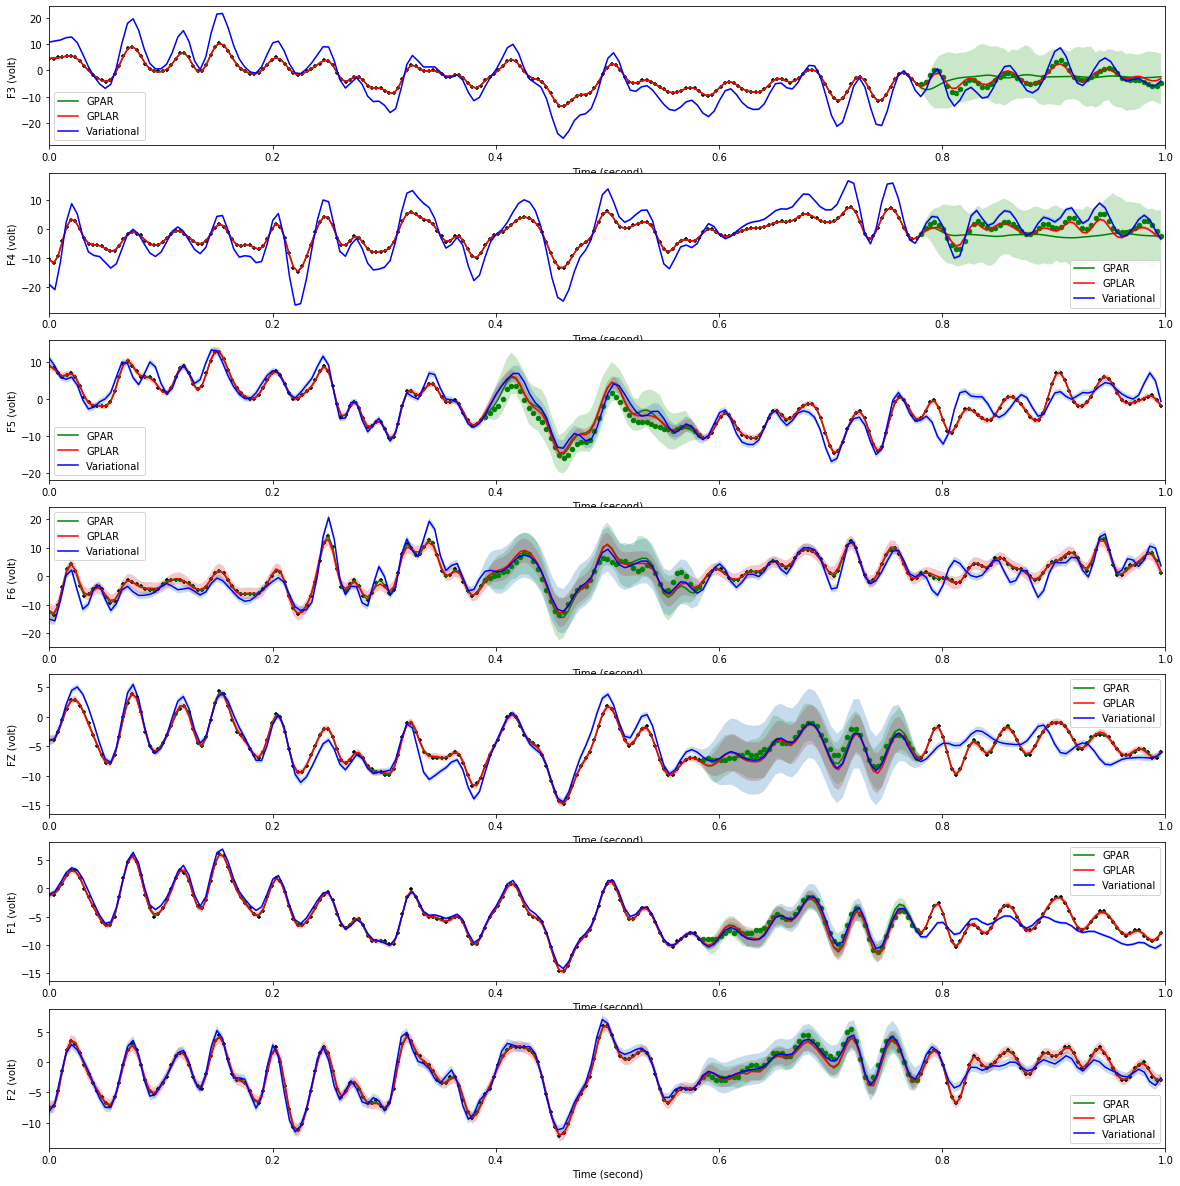
\includegraphics[width=.8\linewidth]{eeg-bidirectional-4.png}
\caption{Containing both close-upwards, close-downwards and middle-open observations}
\end{figure}

\newpage
2. I looked into a case where predictions using close-upwards observations does not have under-estimated uncertainty. It seems like when there is no strong dependency discovered with any of the following observed outputs, (F2 in this example), GPLAR will have large uncertainty and the predicted mean will be corrected by the DGP in reverse.\\


\begin{center}
\begin{tabular}{c|c|l|c}
	\hline
	Output & Time kernel variance & Output Linear kernel variances & Output Non-linear kernel variances\\
	\hline
	FZ & 4.78\\
	\hline
	F1 & 0.36 & FZ:0.711  & 2e-06\\
	\hline
	F2 & 0.31 &  \makecell{FZ:2.4\\F1:0.21} & 4e-06\\
	\hline
	F3 & 0.60 &  \makecell{FZ:6e-07\\F1:0.63\\\textcolor{red}{F2:7e-07}} & 6e-07\\
	\hline
	F4 & 1.90 & \makecell{FZ: 3.43\\F1:1.27\\\textcolor{red}{F2:8e-06}\\F3:8e-05} & 1e-06\\
	\hline
	F5 & 0.28 & \makecell{FZ:6e-07\\F1:3e-05\\\textcolor{red}{F2:4e-07}\\F3:0.51\\F4:6e-07} & 1e-06\\
	\hline
	F6 & 0.59 & \makecell{FZ:6e-04\\F1:3e-05\\\textcolor{red}{F2:5e-06}\\F3:4e-07\\F4:0.19\\F5:3e-04} & 1e-06\\
	\hline
\end{tabular}
\end{center}



\begin{figure}[H]
\centering
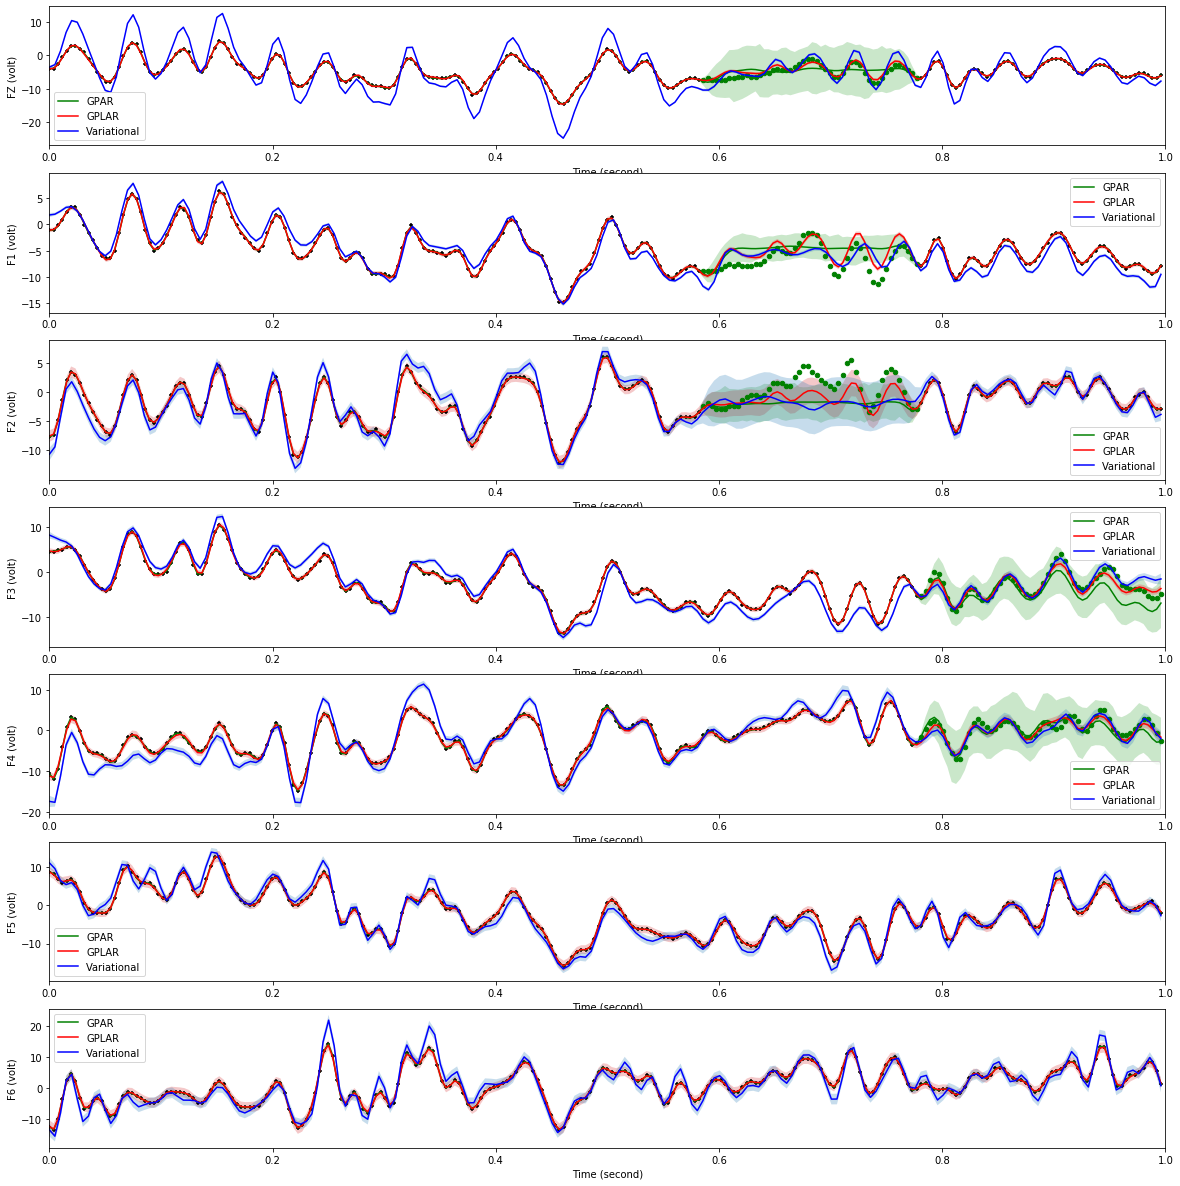
\includegraphics[width=.8\linewidth]{eeg-bidirectional-5.png}
\caption{Uncertainty in F2 is not under-estimated}
\end{figure}

\newpage
3. If DGP in reverse is replaced with another GPLAR in reverse, close-upwards observations can sometimes have ``well-calibrated'' uncertainty as shown below (This dataset is from another patient, no.345), but is not better than gpar or gpar in reverse direction in terms of log-likelihood or smse. If I remove the kernel over time for DGP in reverse, the uncertainty for first three outputs are still underestimated. And ``well-calibrated'' uncertainty is not always maintained, no.346 still has underestimated uncertainty in first two outputs, while no.347 has underestimated uncertainty in the last two outputs. 

\begin{figure}[H]
\centering
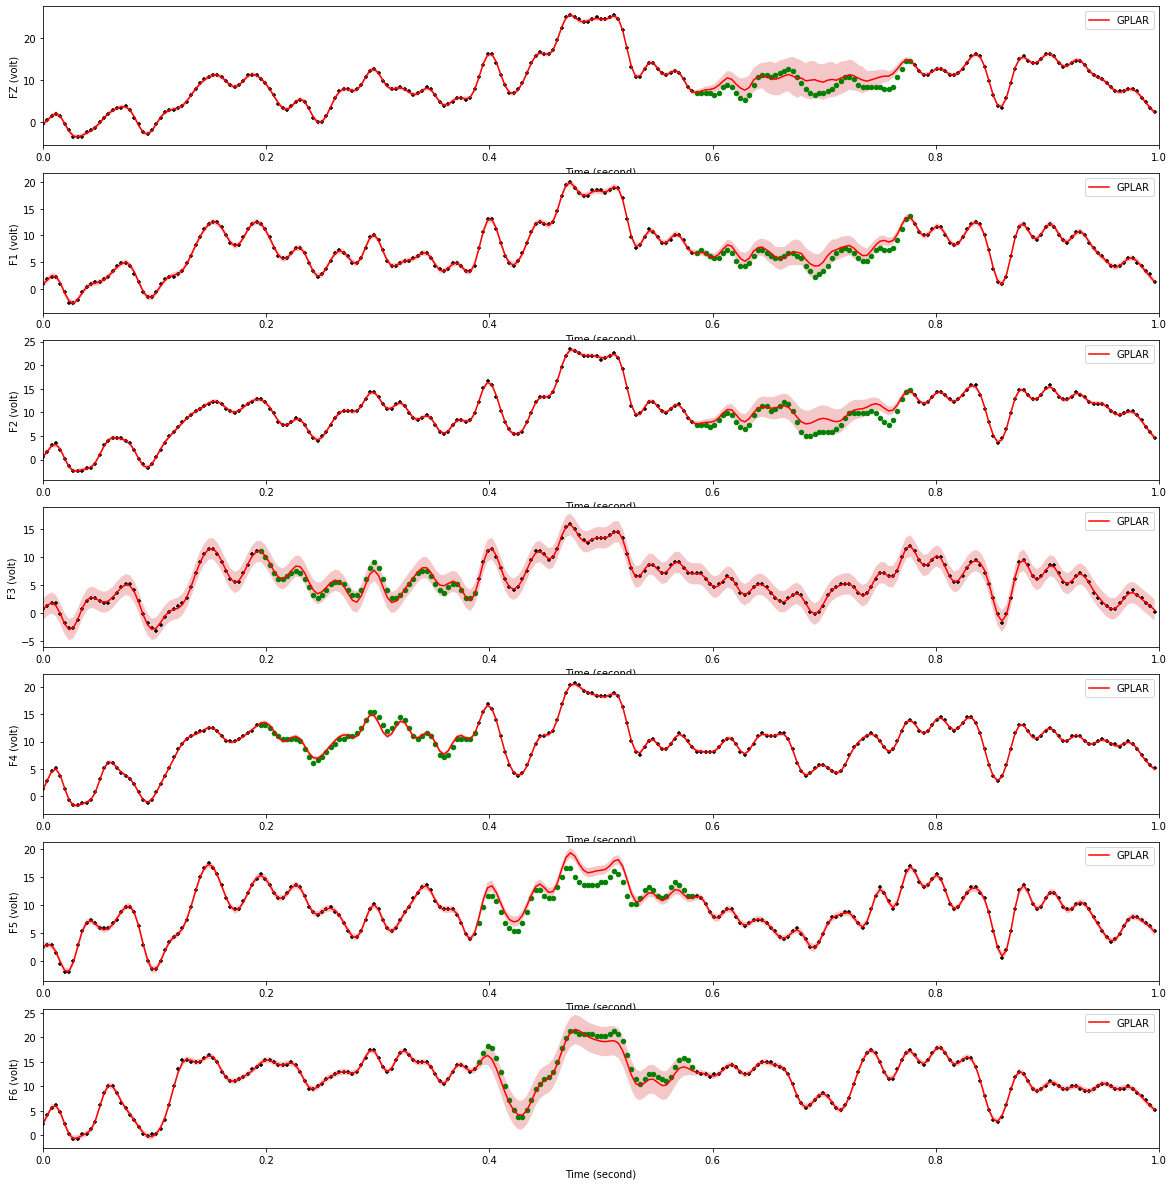
\includegraphics[width=.8\linewidth]{345-eeg-bi-gplar.png}
\caption{Patient No.345 using Bi-GPLAR}
\end{figure}


\begin{figure}[H]
\centering
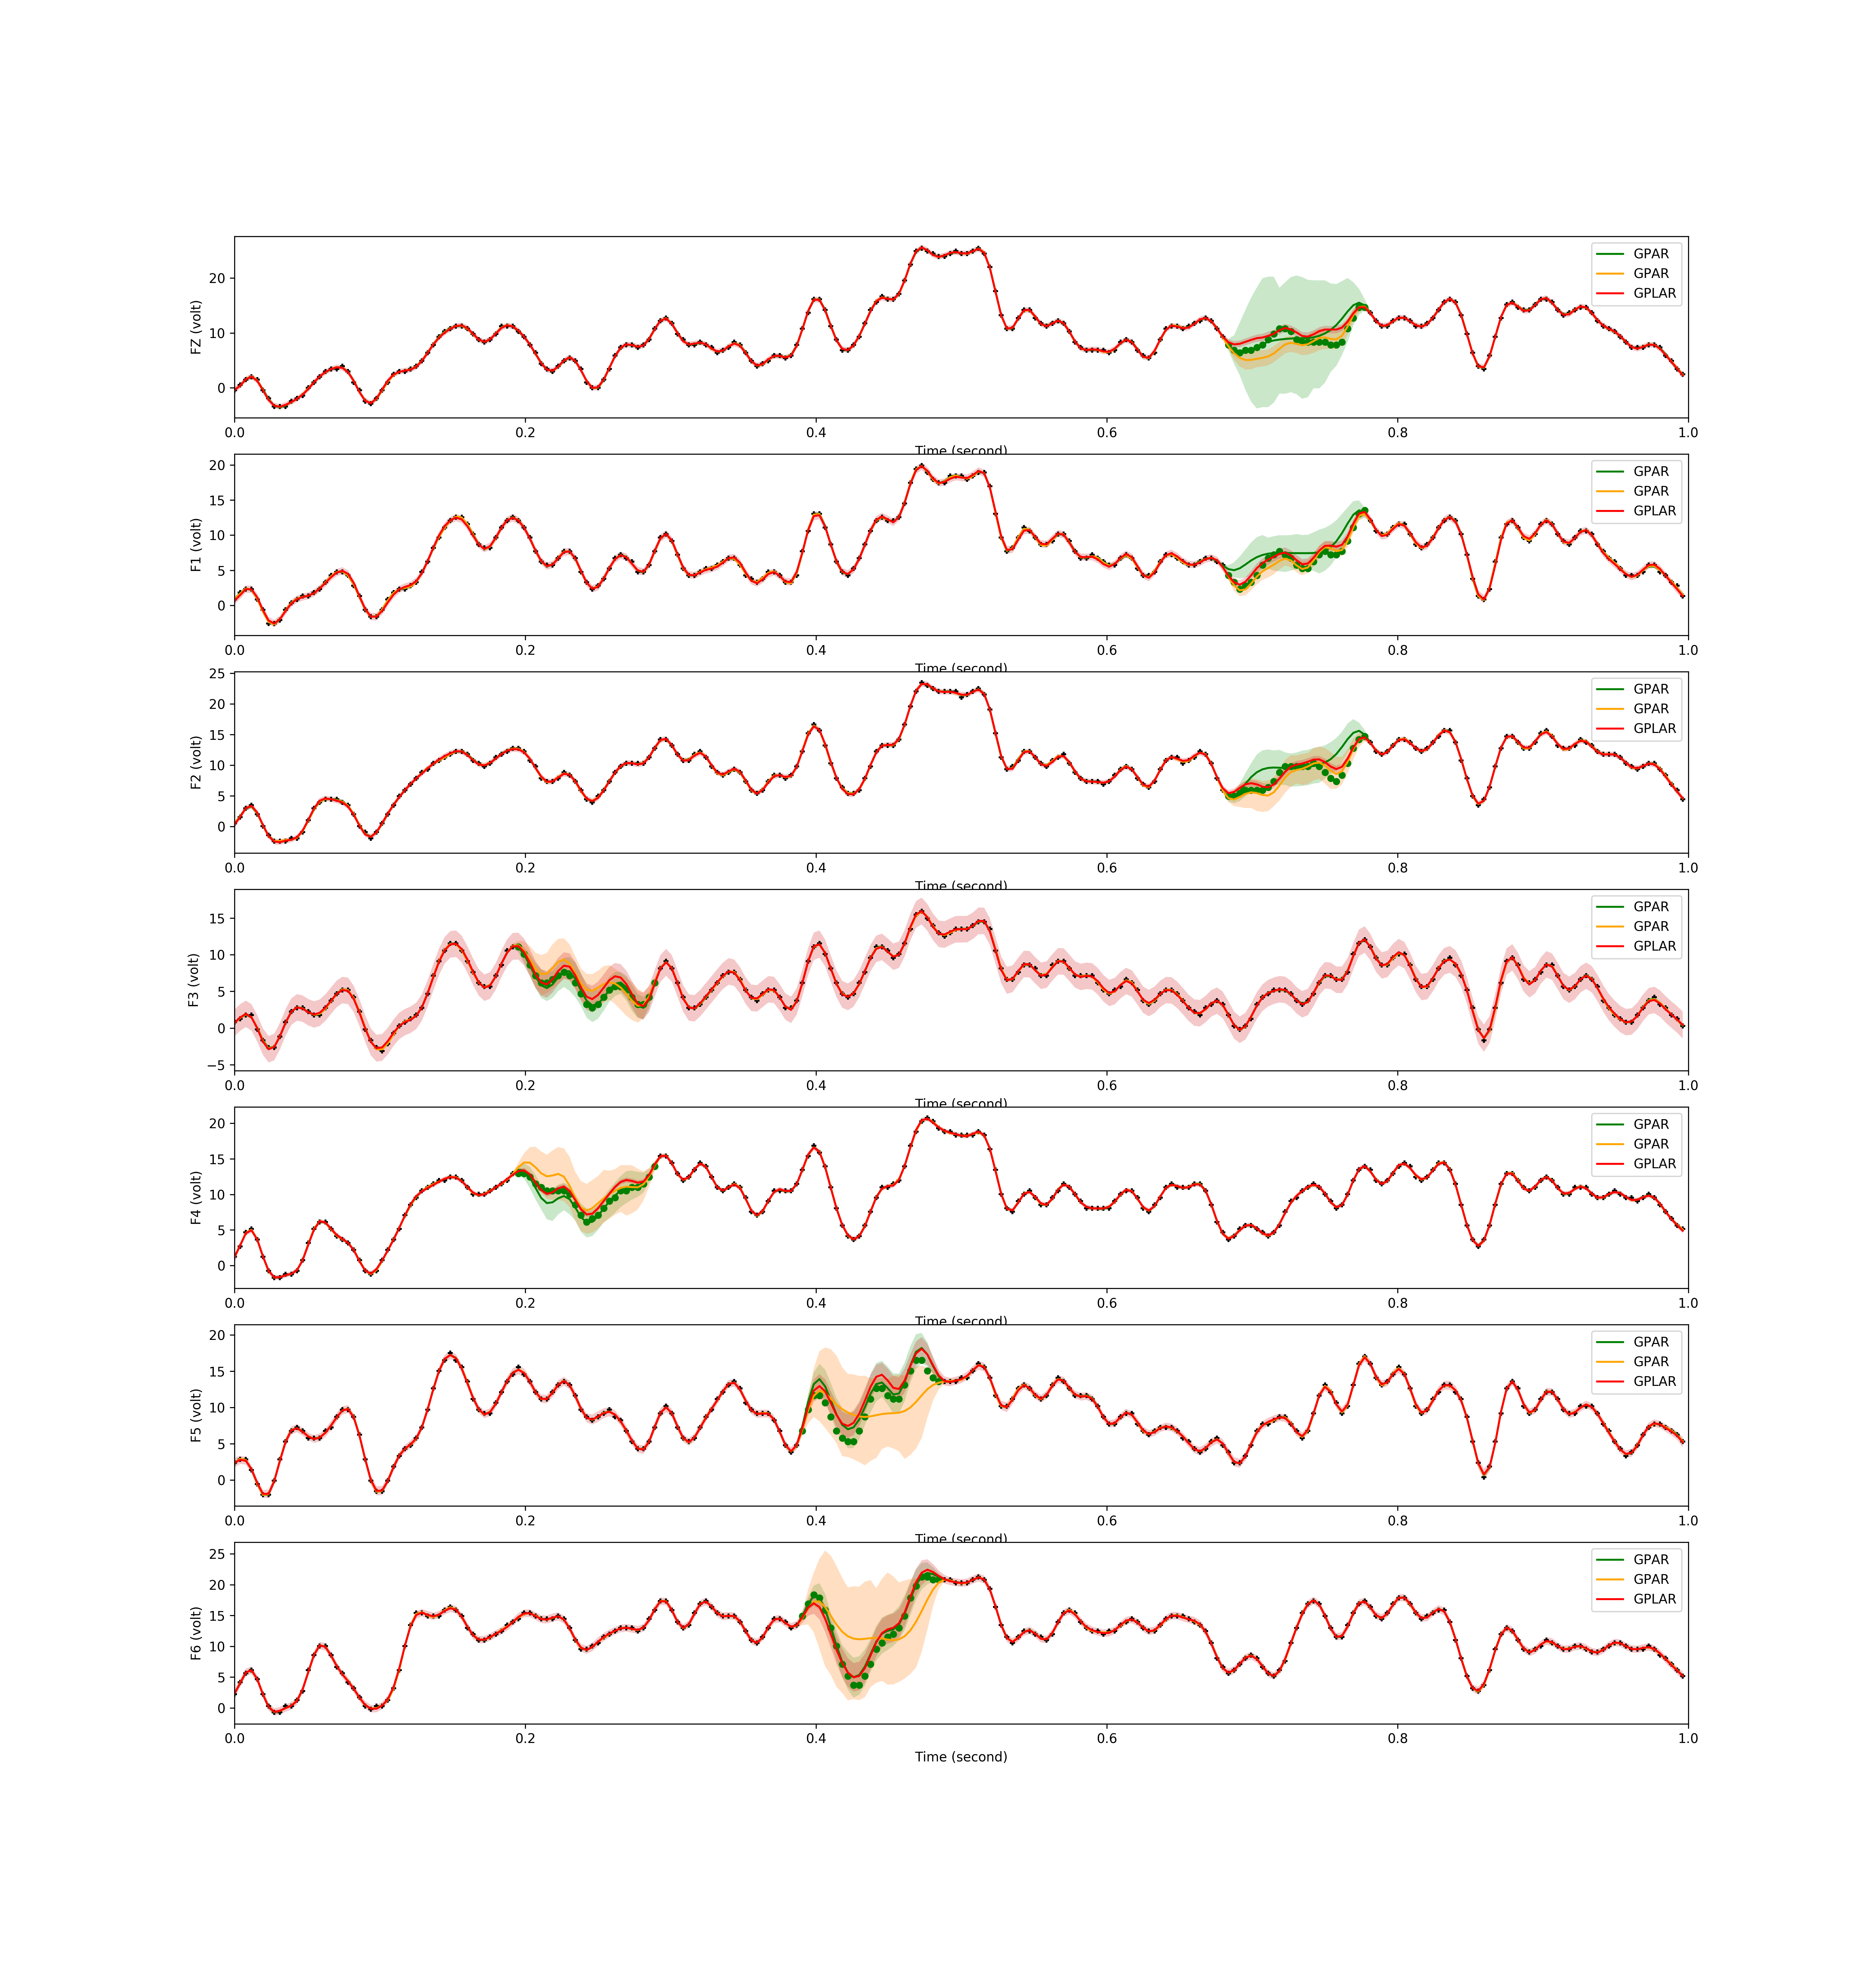
\includegraphics[width=.8\linewidth]{345-eeg-bi-gplar-shorter.png}
\caption{Patient No.345 with shorter missing area using Bi-GPLAR}
\end{figure}


\begin{figure}[H]
\centering
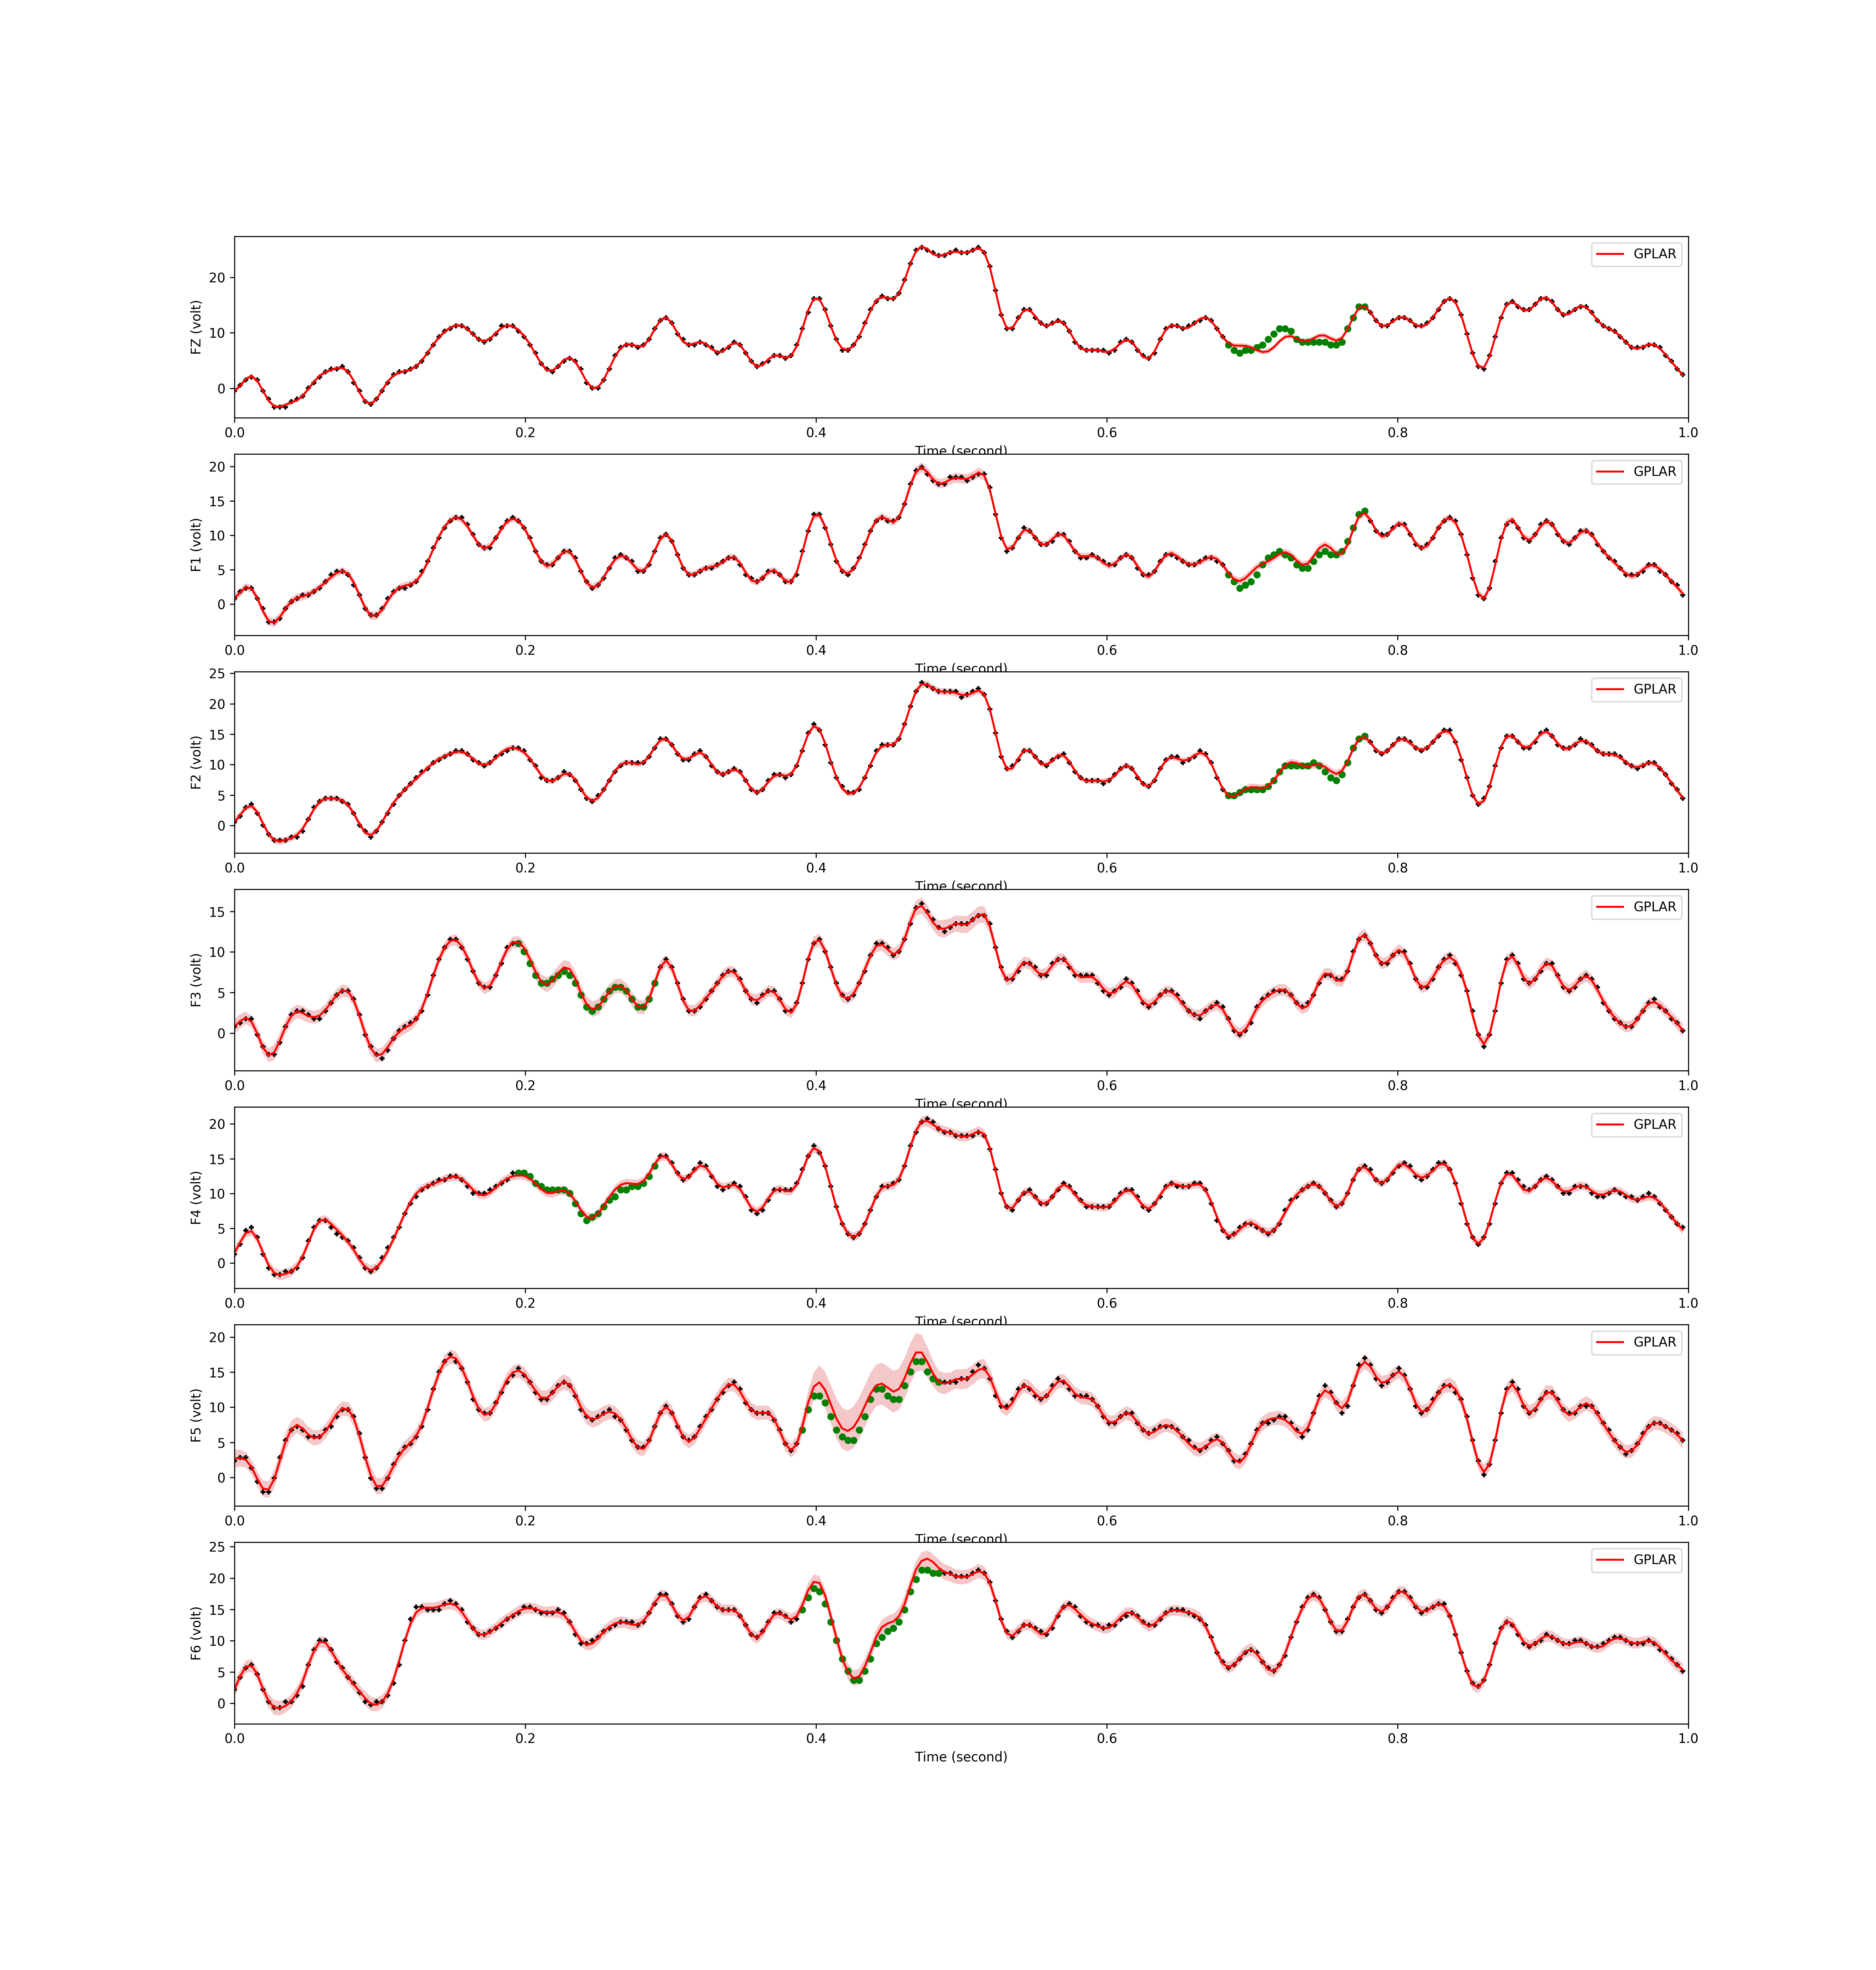
\includegraphics[width=.8\linewidth]{345-eeg-remove-x.png}
\caption{GPLAR + DGP in reverse with time kernel removed}
\end{figure}

\begin{center}
\begin{tabular}{|c|c|c|c|c|c|c|}
	\hline
	 & \multicolumn{3}{c|}{log-likelihood} & \multicolumn{3}{c|}{smse}\\
	\hline
	output & gplar & gpar & gpar-r & gplar & gpar & gpar-r\\
	\hline
	FZ & -622.1 & \textbf{-59.69} & -145.3 & \textbf{0.2473} & 0.4062 & 0.5754\\
	F1 & -196.4 & -60.33 & \textbf{-34.98} & 0.0597 & 0.3949 & \textbf{0.0422}\\
	F2 & -42.67 & -76.34 & \textbf{-37.17} & \textbf{0.0297} & 0.6600 & 0.1322\\
	F3 & \textbf{-6.245} & -20.43 & -55.52 & 0.0293 & \textbf{0.0233} & 0.4367\\
	F4 & -86.05 & \textbf{-25.43} & -62.93 & \textbf{0.0529} & 0.0779 & 0.5360\\
	F5 & \textbf{-41.07} & -60.58 & -50.71 & \textbf{0.1605} & 0.2360 & 0.7496\\
	F6 & -63.48 & \textbf{-32.88} & -117.8 & 0.0440 & \textbf{0.0192} & 0.4358\\
	\hline
\end{tabular}
\end{center}




\begin{figure}[H]
\centering
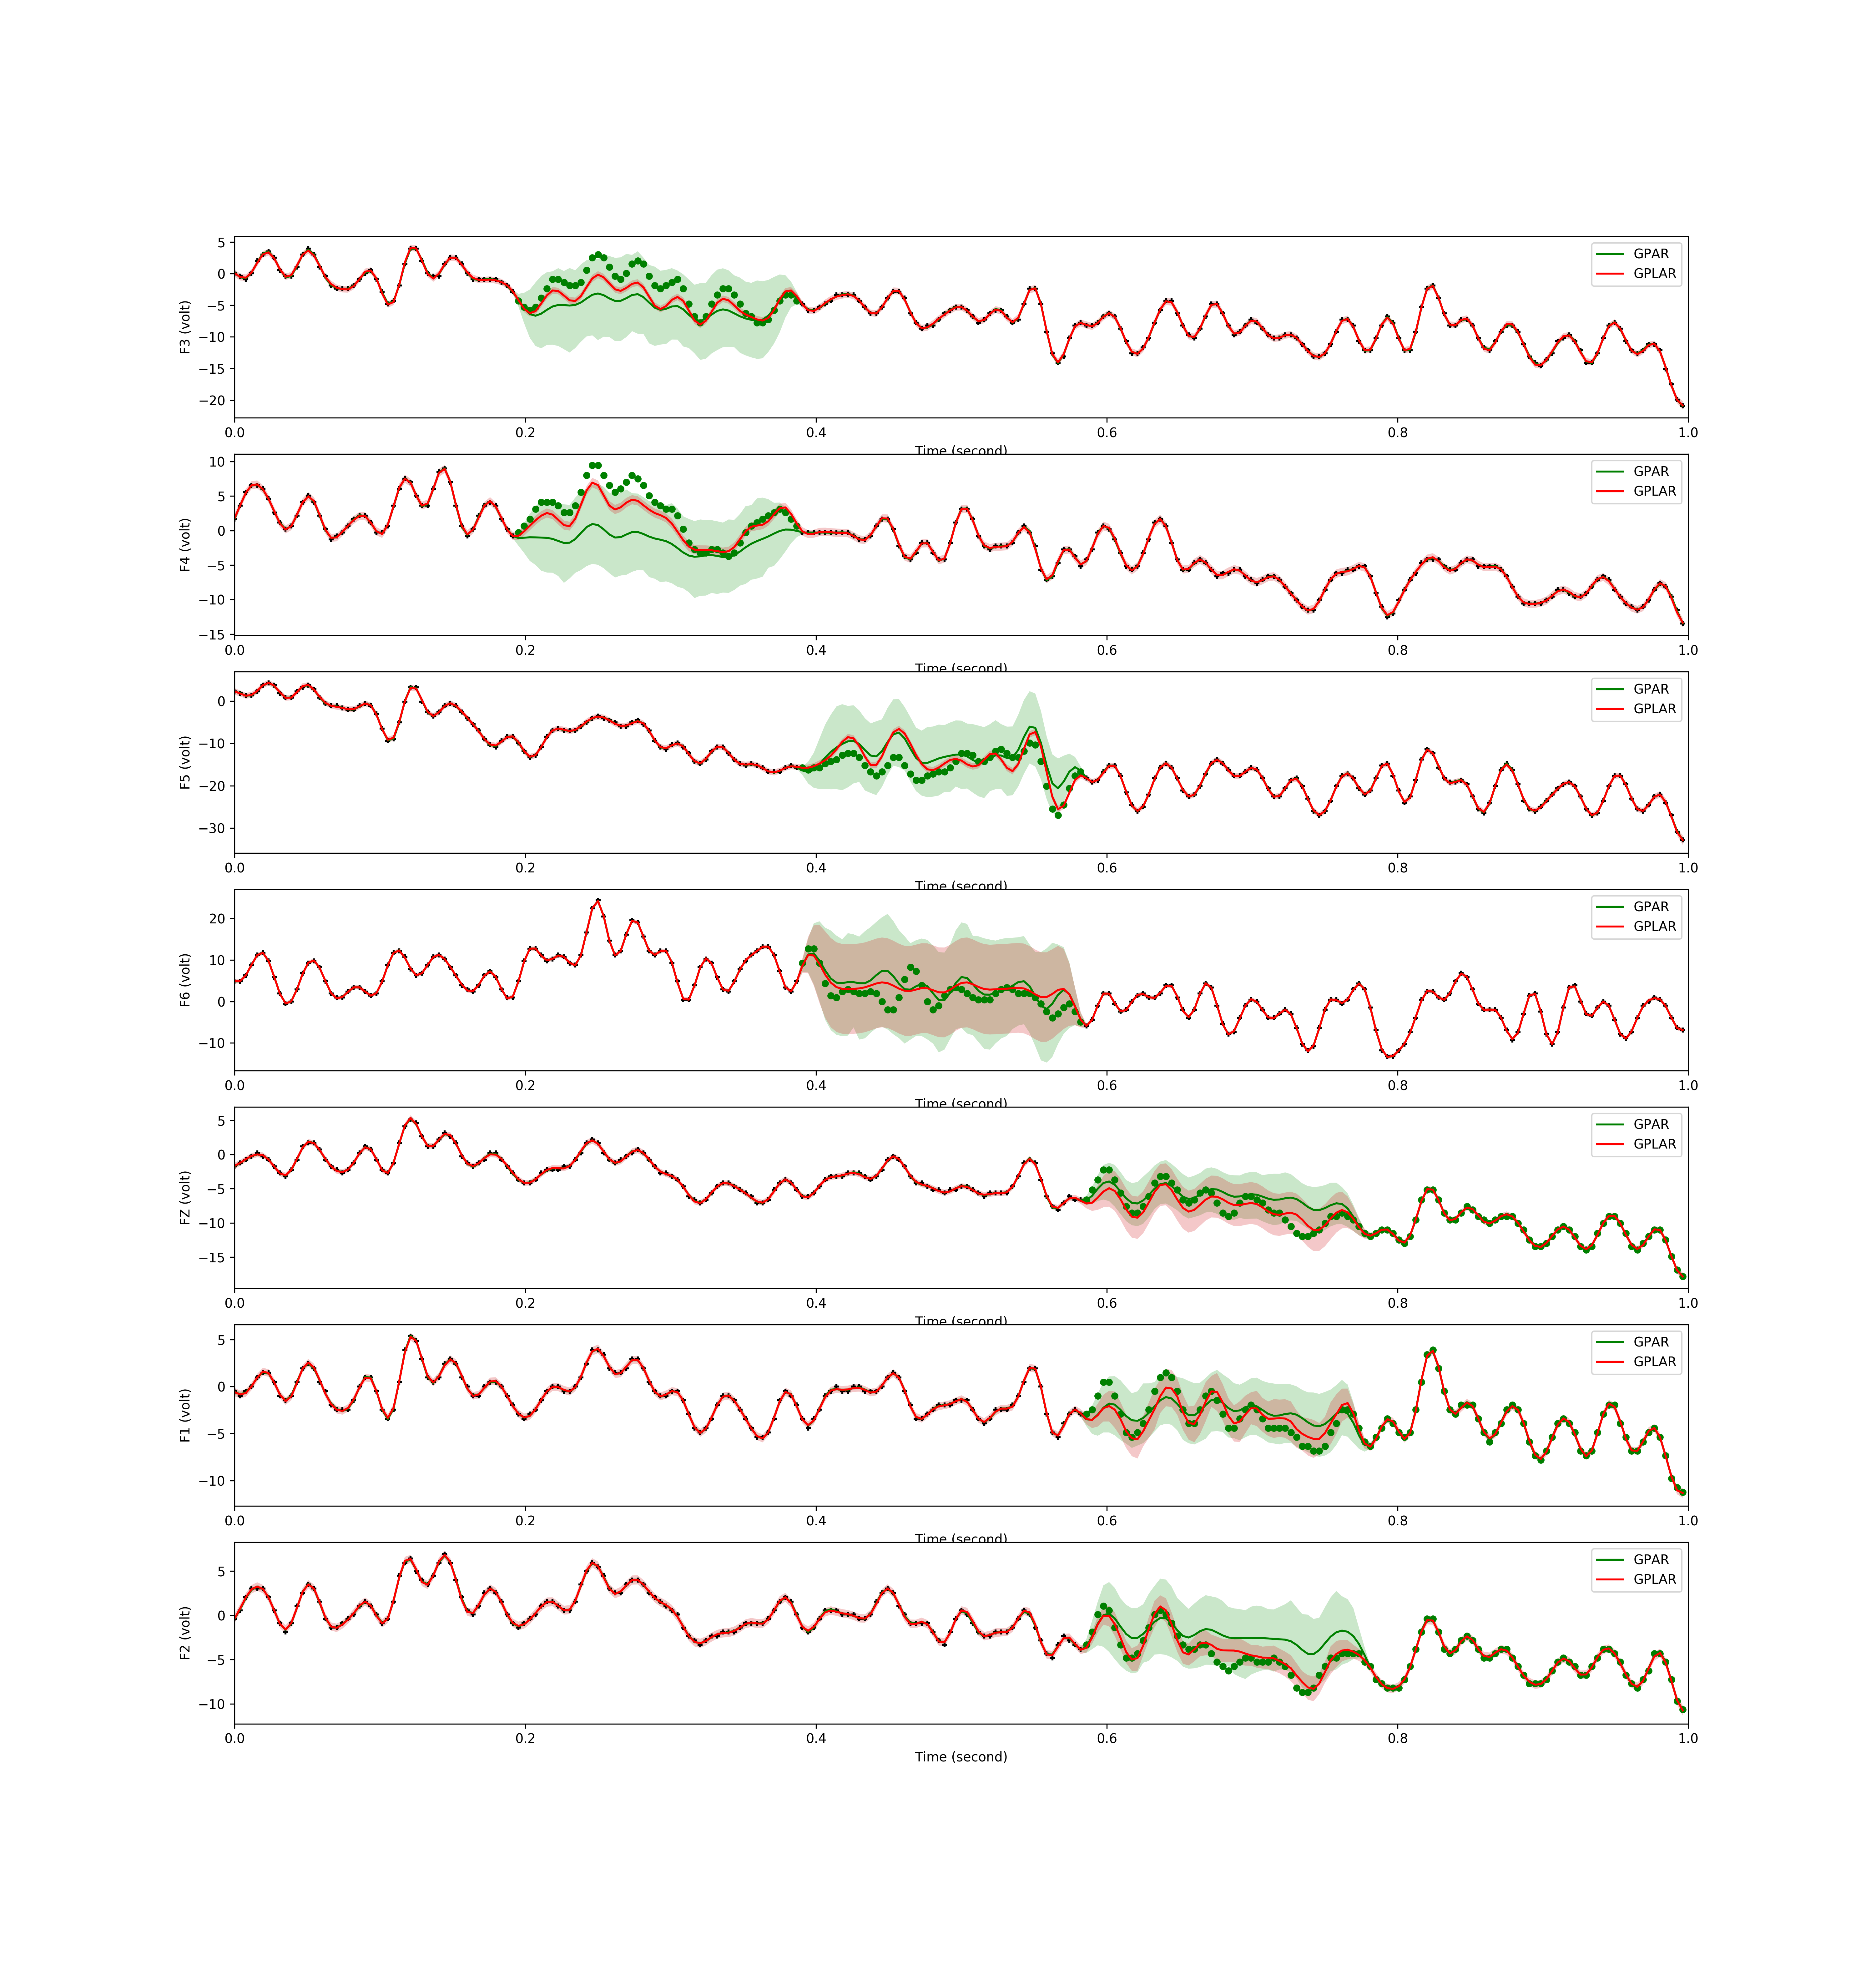
\includegraphics[width=.8\linewidth]{346-eeg-bi-gplar.png}
\caption{Patient No.346}
\end{figure}

\begin{figure}[H]
\centering
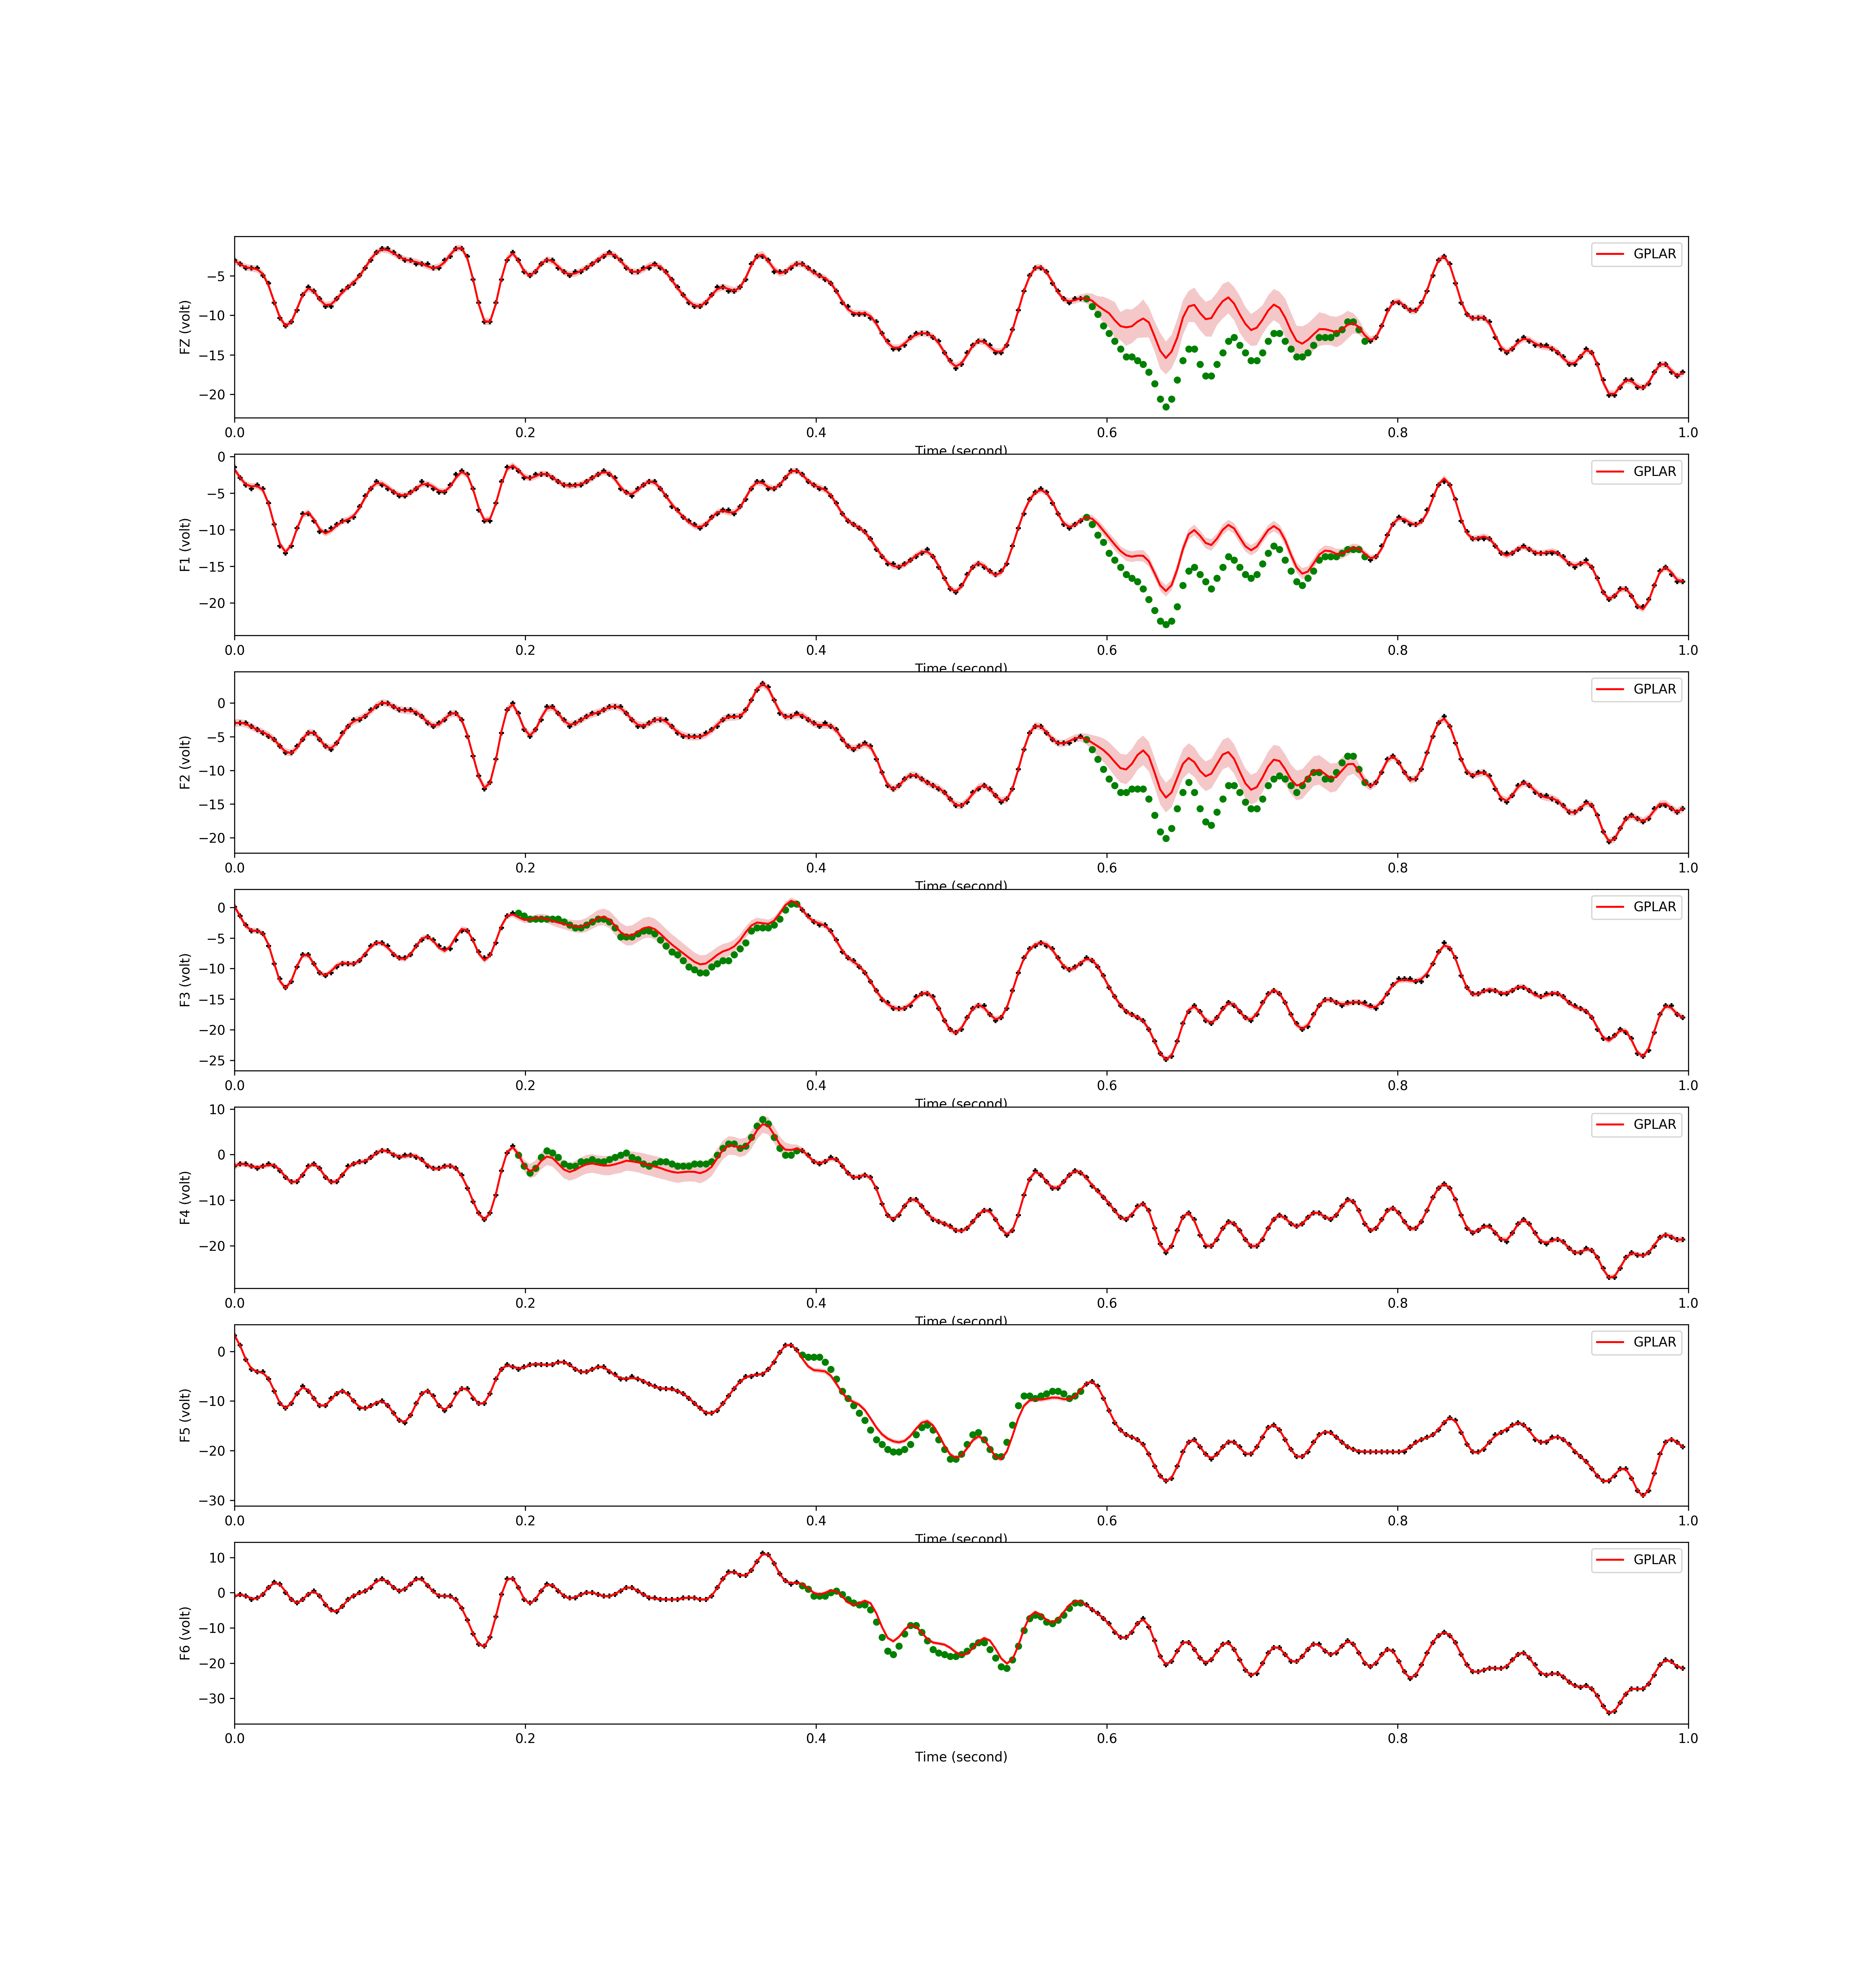
\includegraphics[width=.8\linewidth]{347-eeg-bi-gplar.png}
\caption{Patient No.347}
\end{figure}

\newpage
\begin{figure}[H]
\centering
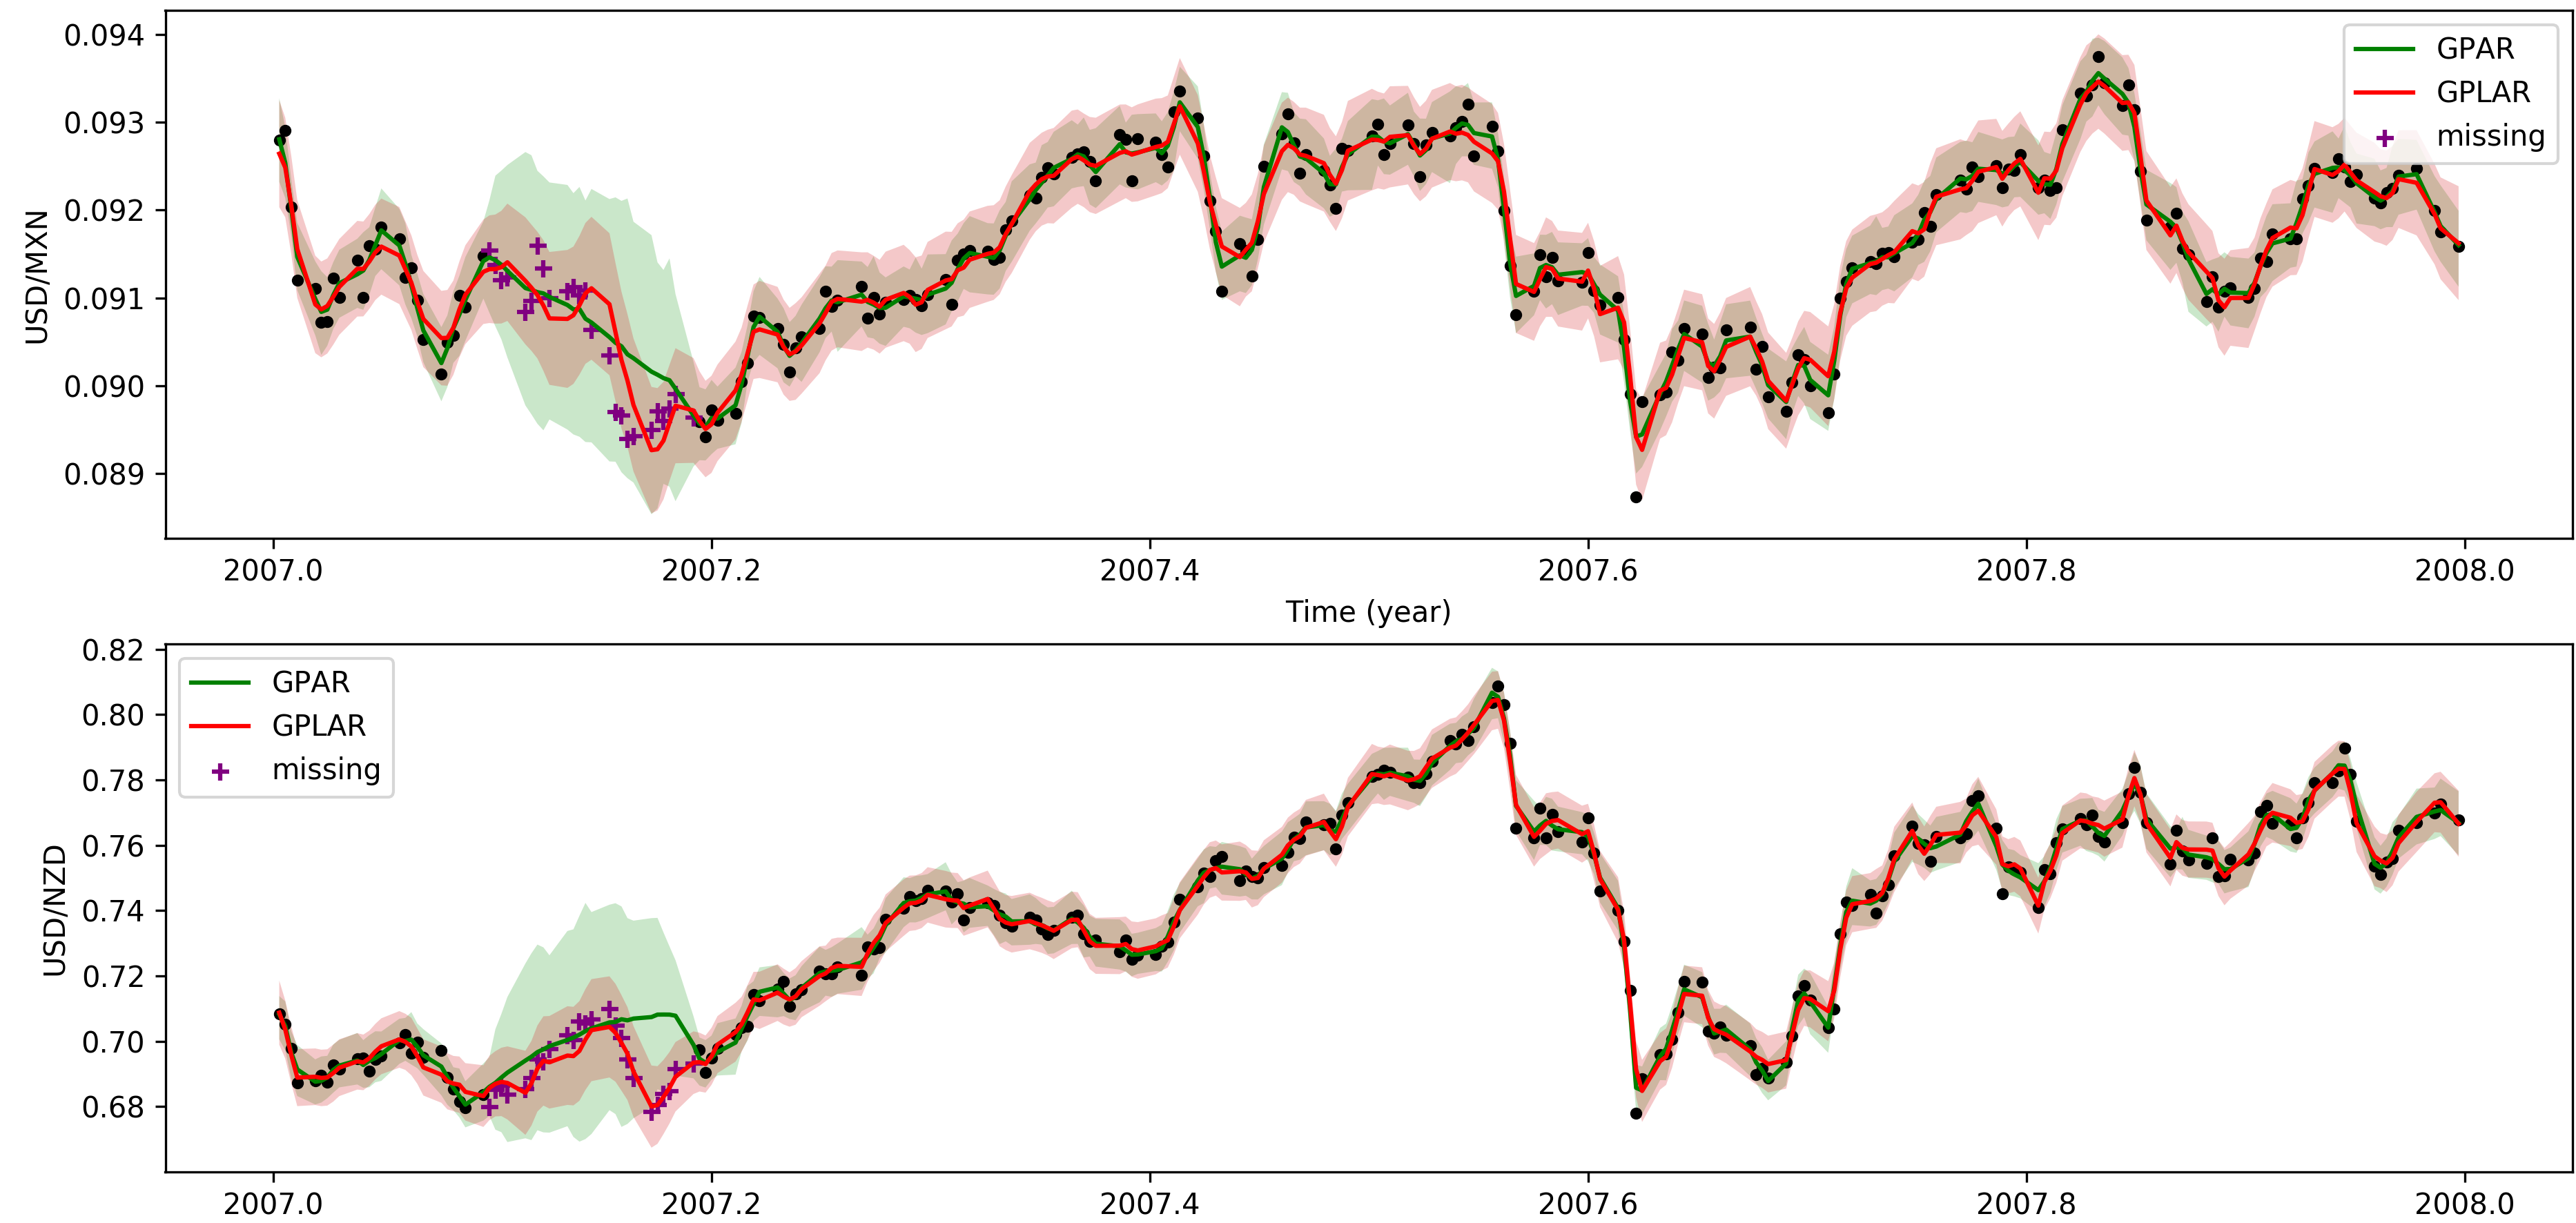
\includegraphics[width=.6\linewidth]{exchange-bi.png}
\caption{I tried smaller missing area on exchange-rate dataset using GPLAR in both direction}
\end{figure}

\begin{figure}[H]
\centering
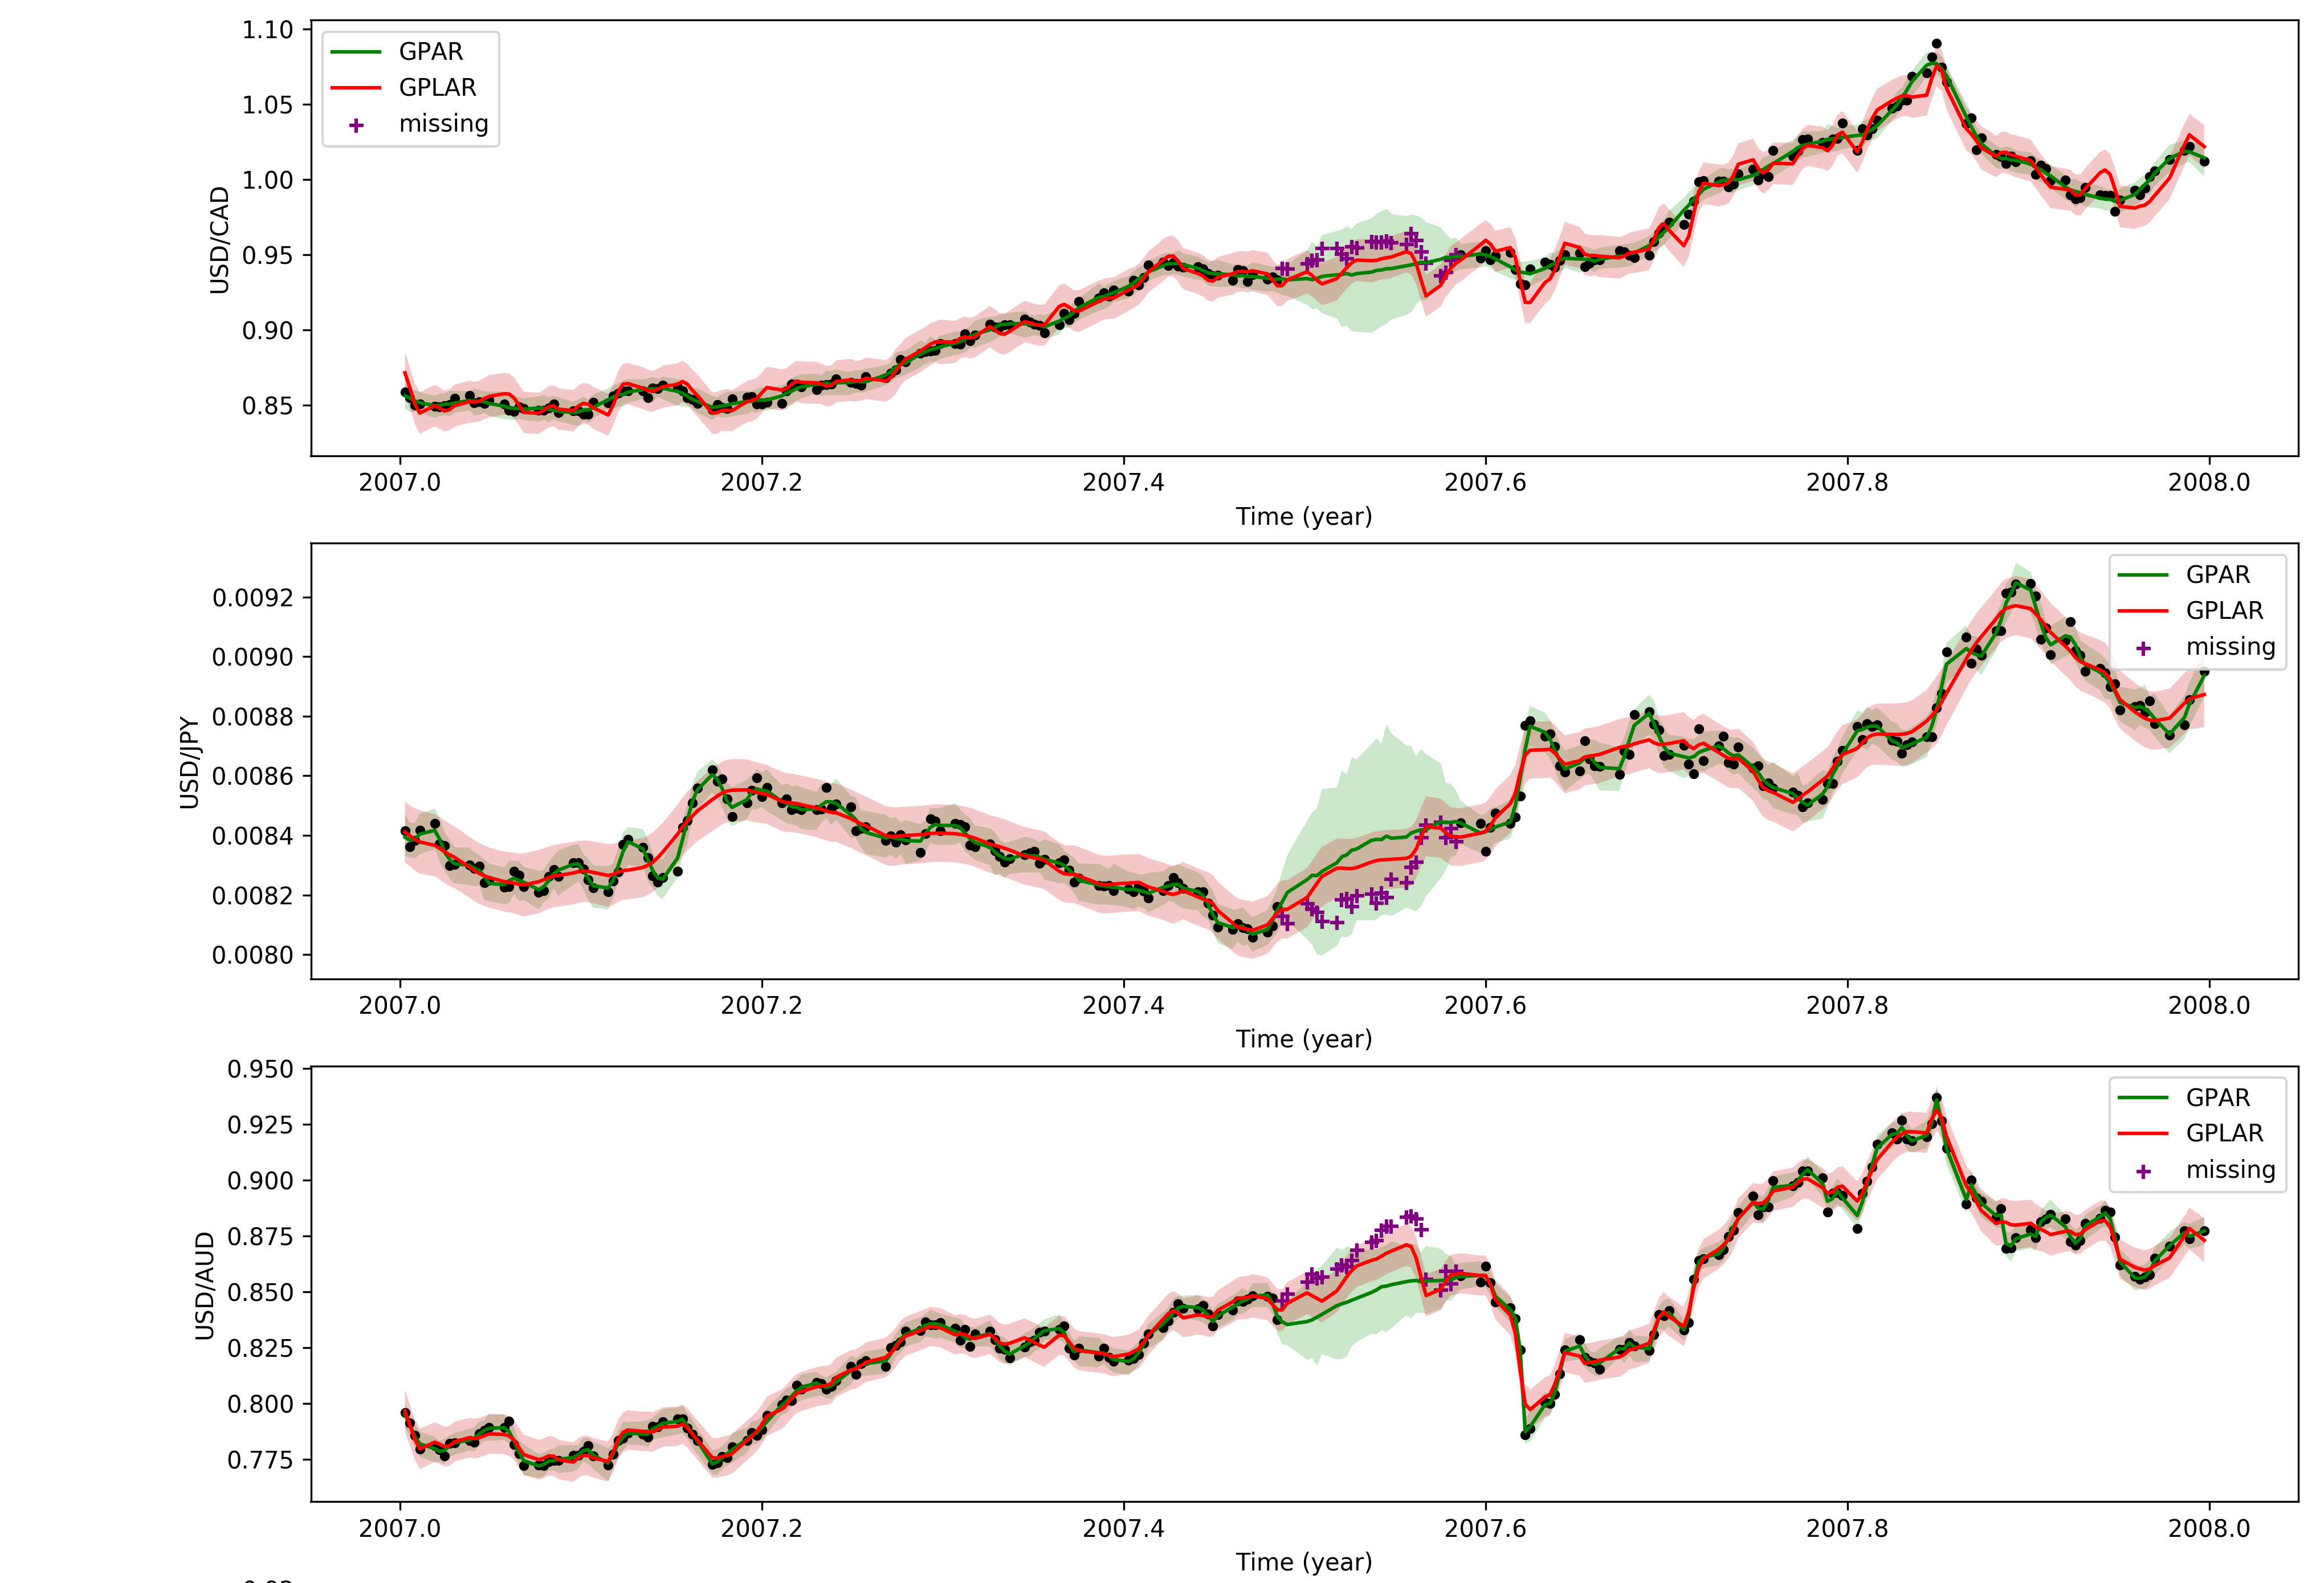
\includegraphics[width=.8\linewidth]{exchange-1.png}
\caption{Some more experiment with close-upwards observations}
\end{figure}

\begin{figure}[H]
\centering
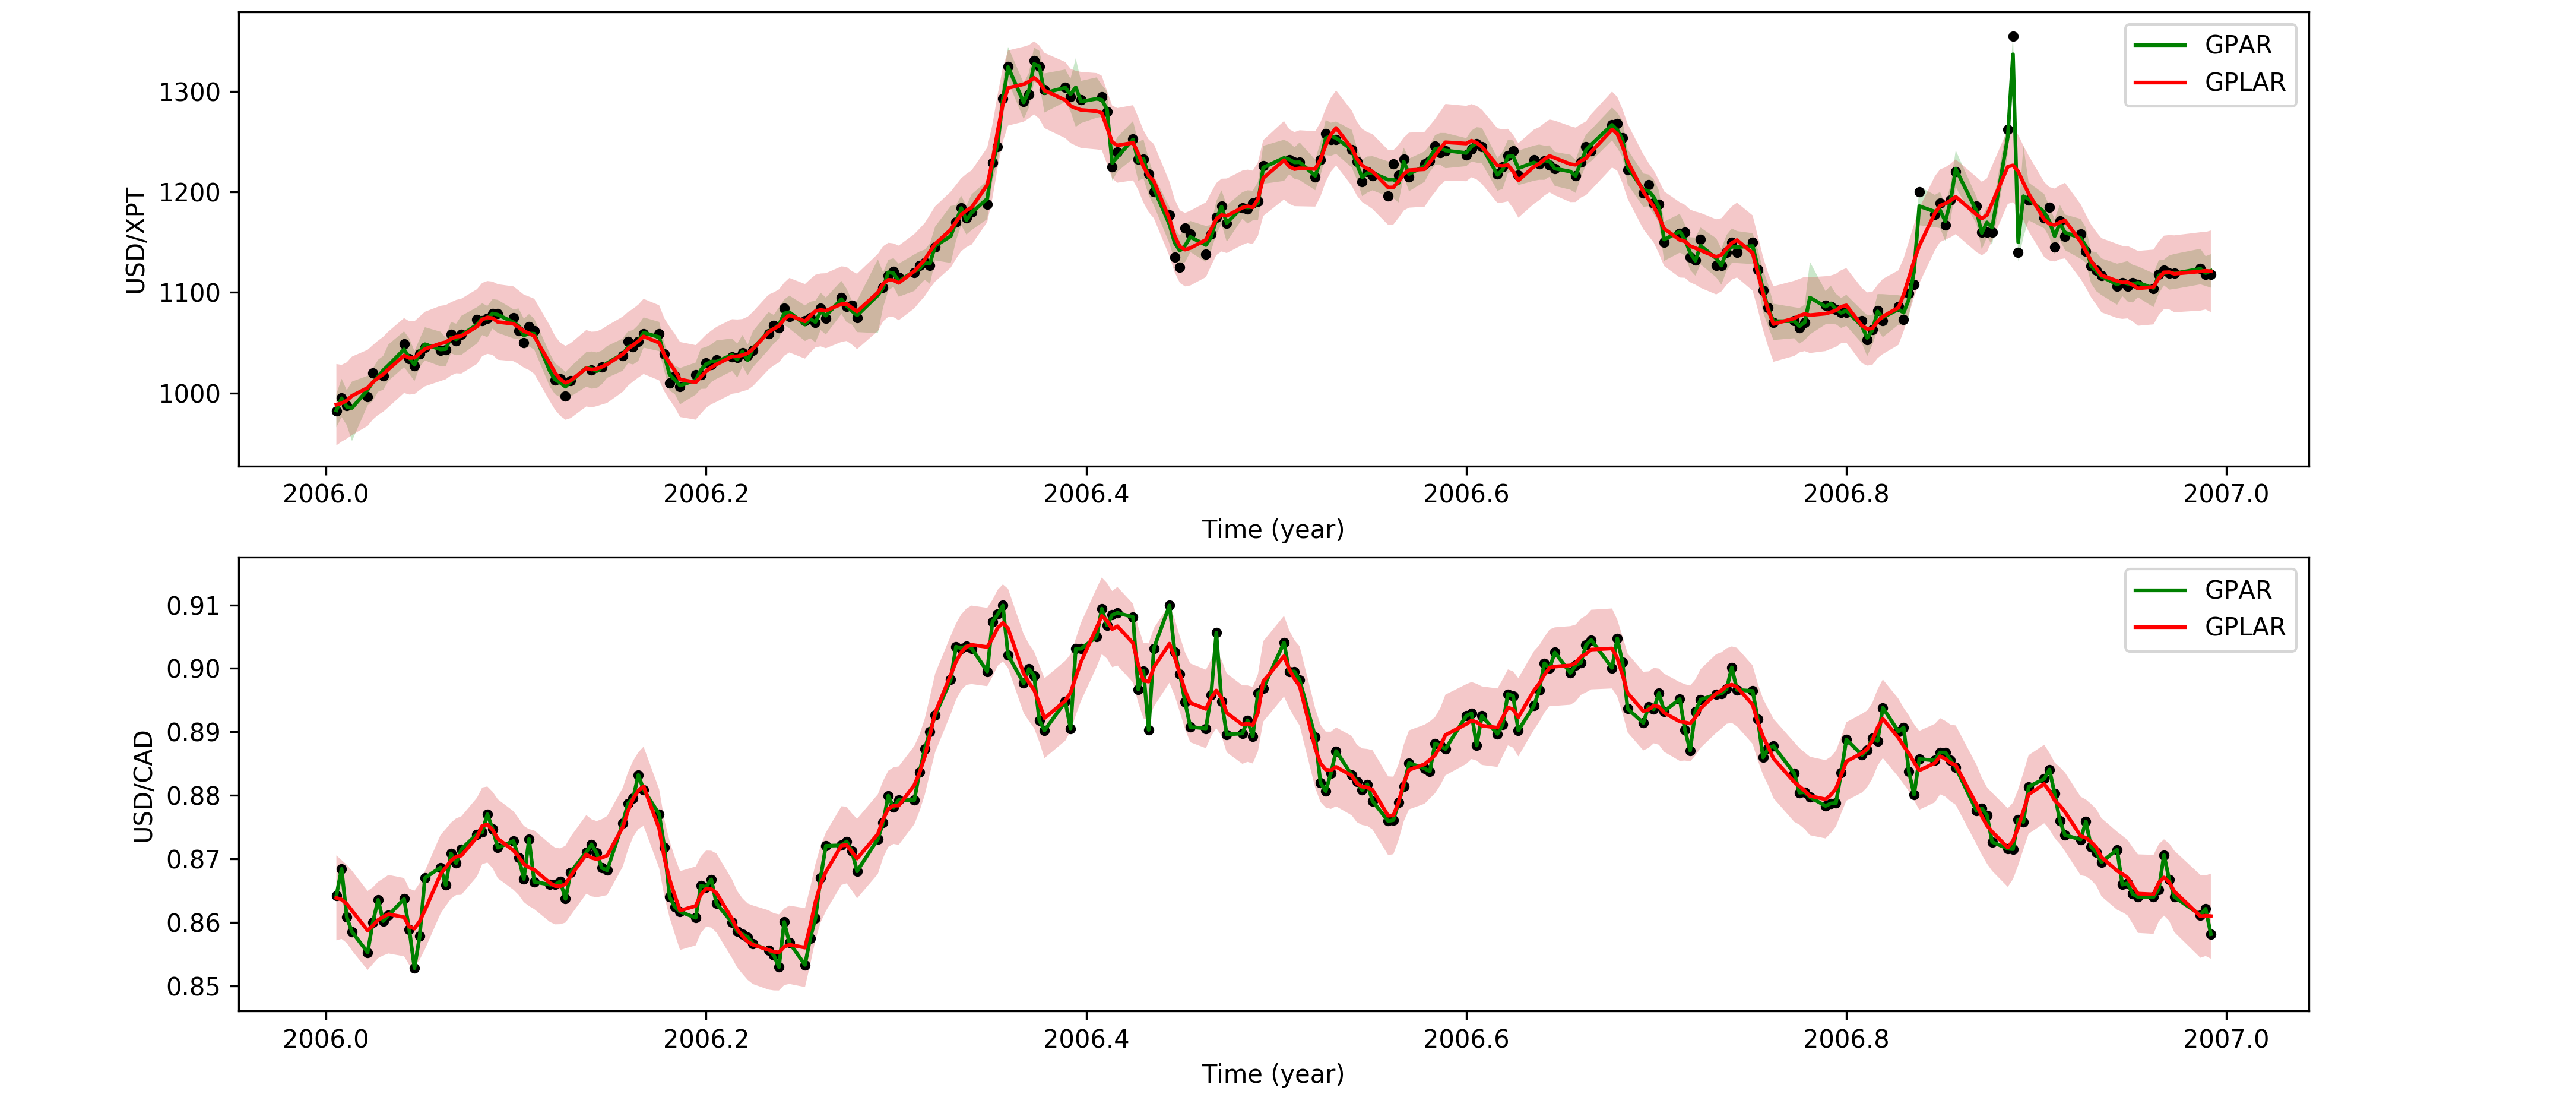
\includegraphics[width=.8\linewidth]{exchange-bi-2006.png}
\caption{Some interesting behaviour on 2006 datasets}
\end{figure}

\begin{figure}[H]
\centering
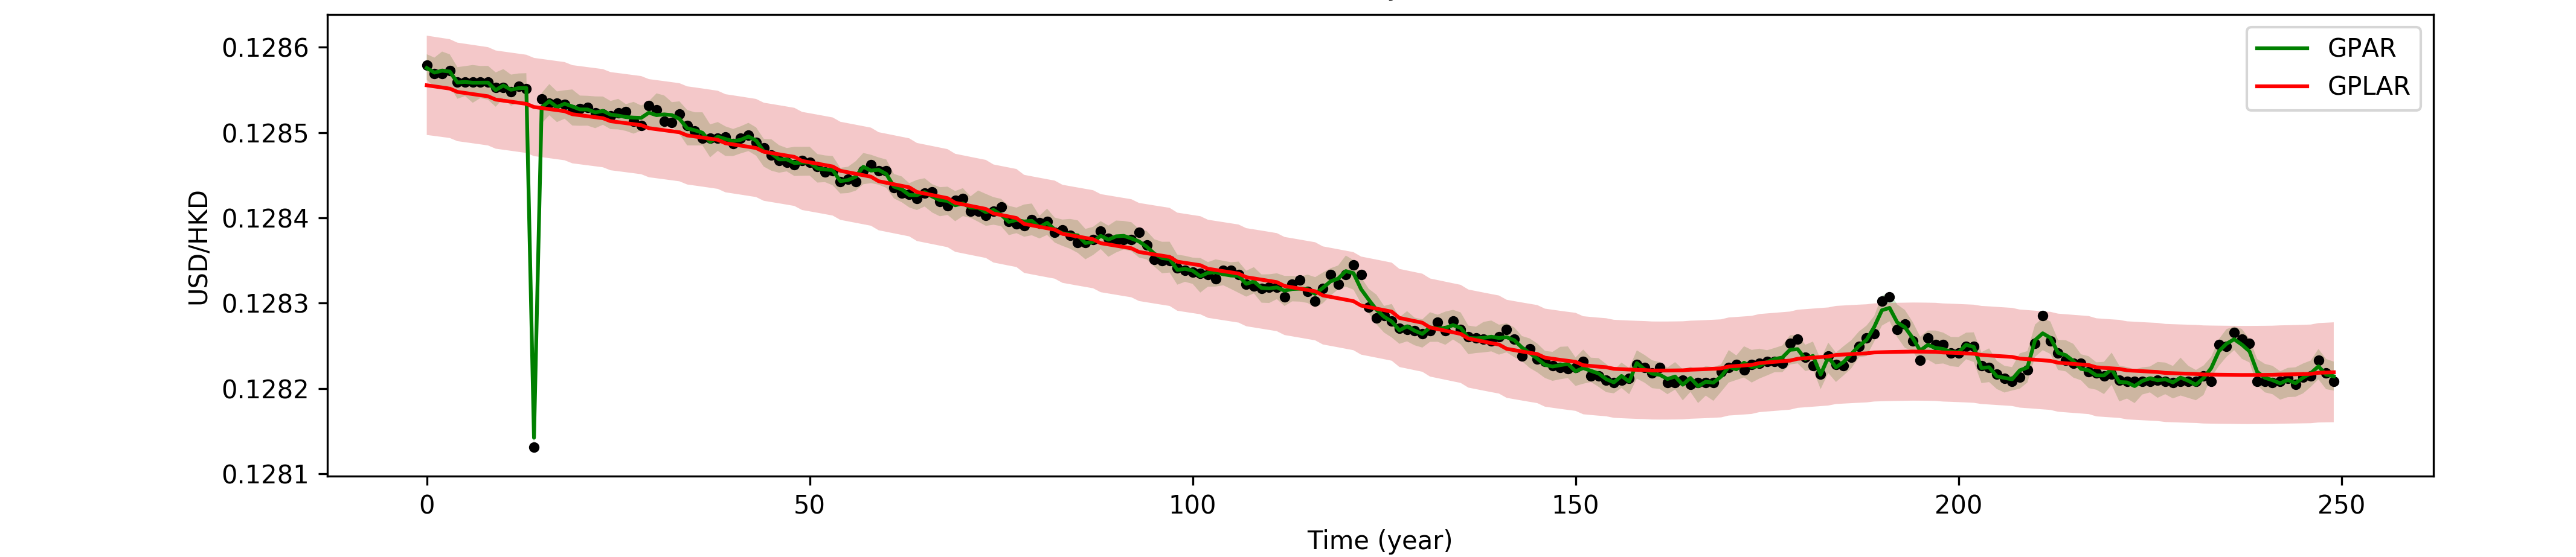
\includegraphics[width=.8\linewidth]{exchange-2000.png}
\caption{Some interesting behaviour on 2000 datasets}
\end{figure}

It is possible that GPAR will be over-fitted to outliers, however, GPLAR might also underfit as shown in Figure 11. We can observe in this exchange-rate dataset that GPAR tends to fit data by more fluctuations, smaller length-scales in kernels, while GPLAR will cover data by increasing the observation noise. 

\newpage
In multi-fidelity model, they conduct an experiments such that 2005's data is considered as low-fidelity input while 2015's data is considered as high-fidelity. I did the same with exchange-rate datasets, collecting USD/GBP data from year 2000-2009, and try to predict some missing values in 2009. For every year, the input ``time'' will be different. However, it seems like the dependencies between years inside same group are rather weak, as shown from the learnt variances value of kernels.

\begin{figure}[H]
\centering
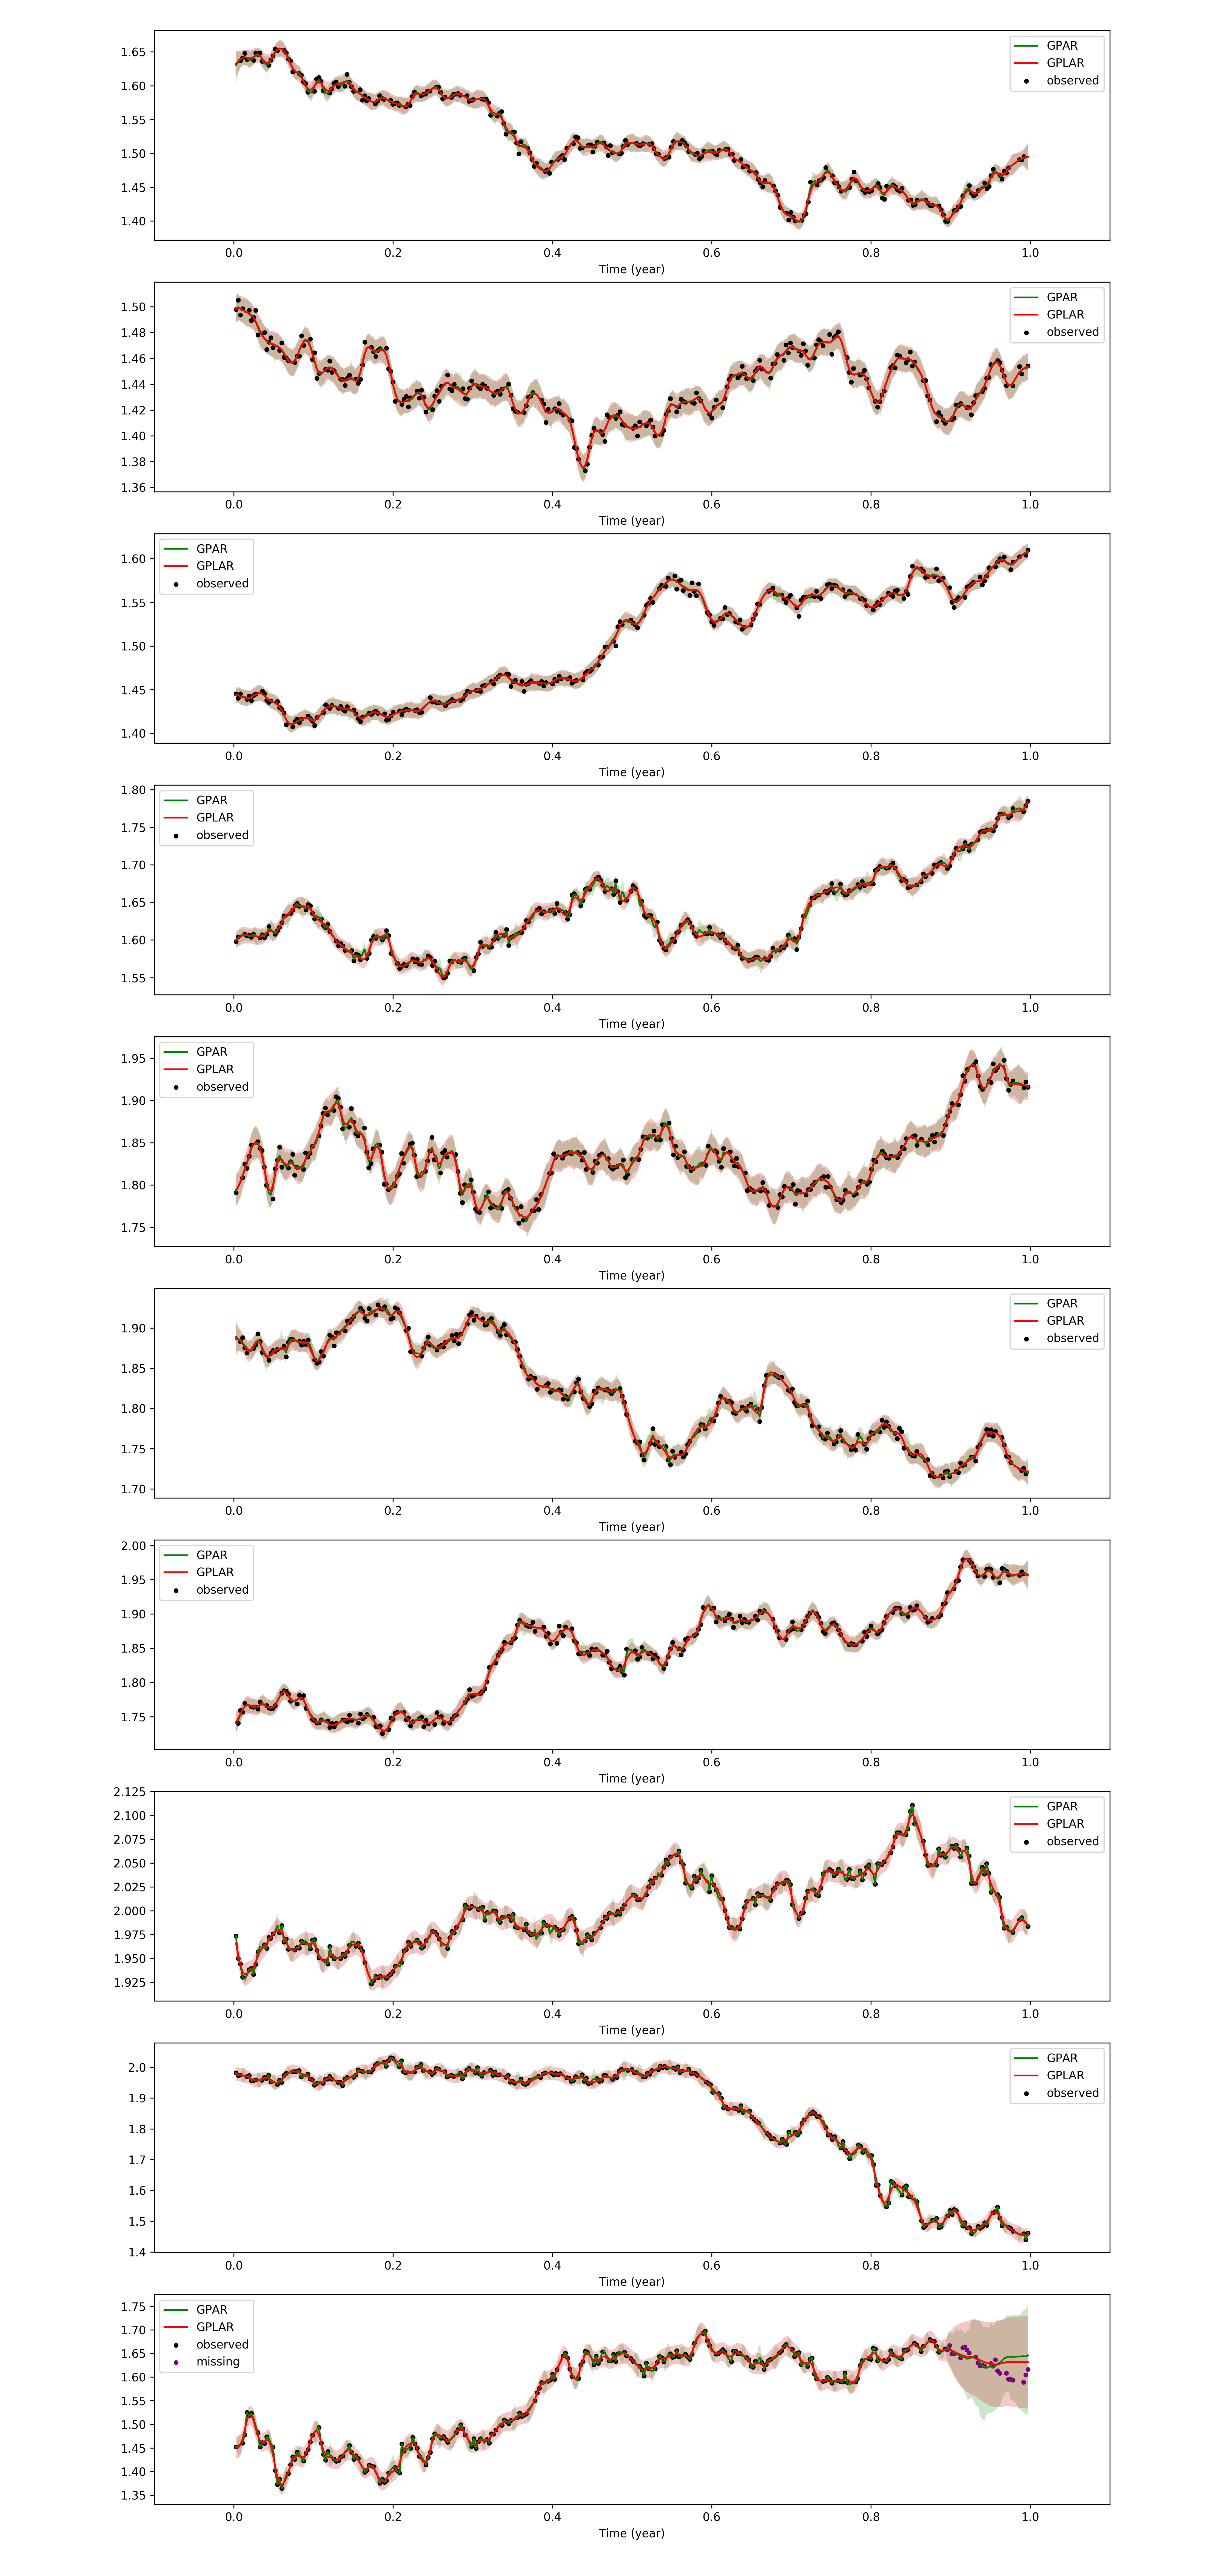
\includegraphics[width=.6\linewidth]{USDGBP-21stcentery.png}
\caption{Some interesting behaviour on 2000 datasets}
\end{figure}

\end{document}
